\documentclass[
    12pt,
    openright,
    oneside,
    a4paper,
    fleqn,
    chapter=TITLE,
    section=TITLE,
    english,
    brazil
]{abntex2}

\usepackage[utf8]{inputenc}
\usepackage[T1]{fontenc}
\usepackage{lmodern}
\usepackage{amsmath,amssymb}
\usepackage{nccmath}
\usepackage{graphicx}
\usepackage{microtype}
\usepackage{indentfirst}
\usepackage{ragged2e}
\usepackage{tabularx,array}
\usepackage{booktabs}
\usepackage{wrapfig}
\usepackage[brazilian,hyperpageref]{backref}
\usepackage[alf]{abntex2cite}
\usepackage{xcolor}

\definecolor{blue}{RGB}{41,5,195}
\definecolor{bitcoin}{HTML}{F7931A}

\setlength{\mathindent}{0pt}
\setlength{\abovedisplayskip}{4pt}
\setlength{\belowdisplayskip}{4pt}
\setlength{\abovedisplayshortskip}{0pt}
\setlength{\belowdisplayshortskip}{0pt}
\setlength{\jot}{3pt}

\newcolumntype{L}[1]{>{\raggedright\arraybackslash}p{#1}}
\newcolumntype{R}{>{\raggedright\arraybackslash}X}
\newenvironment{notacao}[1]{\par\addvspace{6pt}\noindent\tabularx{\linewidth}{@{}L{2.8cm}R@{}}\multicolumn{2}{@{}l}{\textbf{#1}}\\[2pt]}{\endtabularx\par\addvspace{8pt}}

\newcommand{\quadroname}{Quadro}
\newcommand{\listofquadrosname}{Lista de quadros}
\newfloat[chapter]{quadro}{loq}{\quadroname}
\newlistof{listofquadros}{loq}{\listofquadrosname}
\newlistentry{quadro}{loq}{0}
\setfloatadjustment{quadro}{\centering}
\counterwithout{quadro}{chapter}
\renewcommand{\cftquadroname}{\quadroname\space}
\renewcommand*{\cftquadroaftersnum}{\hfill--\hfill}
\setfloatlocations{quadro}{hbtp}
\usepackage{float}

\makeoddhead{abntheadings}{}{}{\ABNTEXfontereduzida\thepage}
\makeevenhead{abntheadings}{\ABNTEXfontereduzida\thepage}{}{}
\makeheadrule{abntheadings}{0pt}{0pt}

\setlength{\parindent}{1.3cm}
\setlength{\parskip}{0.2cm}

\titulo{DIMENSIONAMENTO E SEQUENCIAMENTO DE LOTES DE PRODUÇÃO DE UMA INDÚSTRIA DE BALÕES DE LÁTEX}
\autor{FELIPE PAPA CAPALBO}
\local{SÃO CARLOS - SP}
\data{2026}
\orientador[\textbf{Orientador:}]{Prof. Dr. Victor Claudio Bento de Camargo}
\instituicao{}
\tipotrabalho{Dissertação (Mestrado)}
\preambulo{Dissertação apresentada ao Programa de Pós-Graduação em Engenharia de Produção da Universidade Federal de São Carlos (UFSCar), como parte dos requisitos para obtenção do título de Mestre em Engenharia de Produção.}

\makeatletter
\hypersetup{
    pdftitle={Dimensionamento e sequenciamento de lotes de produção de uma indústria de balões de látex},
    pdfauthor={Felipe Papa Capalbo},
    pdfsubject={\imprimirpreambulo},
    pdfcreator={Felipe Papa Capalbo},
    pdfkeywords={dimensionamento de lotes, sequenciamento da produção, planejamento hierárquico, programação inteira mista, balões de látex},
    colorlinks=true,
    linkcolor=blue,
    citecolor=blue,
    filecolor=magenta,
    urlcolor=blue,
    bookmarksdepth=4
}
\makeatother

\begin{document}

\selectlanguage{brazil}
\frenchspacing
\citeoption{abnt-caixa-mista}

\pretextual

\begin{center}
    {\fontsize{16pt}{16pt}\selectfont \textbf{UNIVERSIDADE FEDERAL DE SÃO CARLOS}}\\[10pt]

    {\fontsize{14pt}{14pt}\selectfont CENTRO DE CIÊNCIAS EXATAS E DE TECNOLOGIA}\\[10pt]

    {\fontsize{14pt}{14pt}\selectfont PROGRAMA DE PÓS-GRADUAÇÃO EM ENGENHARIA DE PRODUÇÃO}\\

    \vspace*{\fill}

    
\includegraphics[width=0.8\textwidth]{figuras/UFSCar.png}

    \vspace*{\fill}

    {\fontsize{14pt}{14pt}\selectfont \textbf{\imprimirtitulo}}\\

    \vspace*{\fill}

    {\fontsize{14pt}{14pt}\selectfont Felipe Papa Capalbo}\\

    \vspace*{\fill}

    {\fontsize{12pt}{12pt}\selectfont \textbf{DISSERTAÇÃO DE MESTRADO EM ENGENHARIA DE PRODUÇÃO}}

    \vspace*{\fill}
\end{center}

\cleardoublepage

\imprimirfolhaderosto

\begin{fichacatalografica}
    \vspace*{\fill}
    \begin{center}
        [FICHA CATALOGRÁFICA GERADA PELA BIBLIOTECA COMUNITÁRIA DA UFSCAR]
    \end{center}
    \vspace*{\fill}
\end{fichacatalografica}

\begin{folhadeaprovacao}
    \vspace*{\fill}
    \begin{center}
        [FOLHA DE APROVAÇÃO ASSINADA PELA BANCA]
    \end{center}
    \vspace*{\fill}
\end{folhadeaprovacao}

\cleardoublepage
\vspace*{\fill}
\begin{flushright}
    \begin{minipage}{0.6\textwidth}
        \justifying
        \textbf{Dedico} [A ESCREVER].
    \end{minipage}
\end{flushright}

\cleardoublepage
\vspace*{\fill}
\begin{flushright}
    \begin{minipage}{0.6\textwidth}
        \justifying
        \textbf{Agradeço} [A ESCREVER].
    \end{minipage}
\end{flushright}

\cleardoublepage
\vspace*{\fill}
\begin{flushright}
    \begin{minipage}{0.6\textwidth}
        \justifying
        [EPÍGRAFE A ESCREVER]
    \end{minipage}
\end{flushright}

\cleardoublepage

\setlength{\absparsep}{18pt}
\begin{resumo}
A produção de balões de látex combina demanda sazonal de calendário, capacidade de moldagem fixa e dois \textit{setups} de escalas distintas: a troca de forma, intervenção mecânica que consome parcela relevante de um turno, e a troca de cor, dependente de sequência e direcional. Este trabalho formula o dimensionamento e sequenciamento de lotes dessa indústria em dois níveis encadeados. O nível semanal é um problema de dimensionamento de lotes capacitado em máquinas paralelas não relacionadas, agregado por balão, que separa a demanda em carteira, cujo atraso é transportado, e previsão líquida da carteira, cuja falta é venda perdida, sobre um estoque único limitado pela capacidade do armazém e protegido por um estoque mínimo nos itens produzidos para estoque. O nível operacional detalha as primeiras semanas do horizonte em turnos, decide a forma montada em cada máquina e as corridas de cada SKU, e recebe do nível semanal uma única informação, a meta de estoque ao fim de cada semana, cobrada como restrição suave. Os dois modelos compartilham a estrutura de objetivo, resolvida em ordem lexicográfica com travas exatas entre estágios: atraso da carteira, venda perdida, violação da meta de estoque e, por fim, custo de \textit{setup} e de carregamento. A ordem das cores dentro de cada turno é decidida por uma heurística de sequenciamento, com cada restrição operacional escrita como equação nomeada, que ocupa a capacidade ociosa deixada pela reserva conservadora de tempo de troca de cor e antecipa produção já planejada sem acrescentar trocas. A previsão de demanda vem de um modelo econométrico hierárquico \textit{top-down}, avaliado fora da amostra pelo erro percentual absoluto médio e pelo viés. [RESULTADOS A ESCREVER]

\textbf{Palavras-chave}: dimensionamento de lotes; sequenciamento da produção; planejamento hierárquico; programação inteira mista; balões de látex.
\end{resumo}

\begin{resumo}[Abstract]
\begin{otherlanguage*}{english}
Latex balloon production combines calendar-driven seasonal demand, fixed moulding capacity and two setups of different scales: the form change, a mechanical intervention that takes a substantial share of a shift, and the colour change, which is sequence-dependent and directional. This work formulates the lot sizing and scheduling problem of this industry in two linked levels. The weekly level is a capacitated lot sizing problem on unrelated parallel machines, aggregated by balloon, that splits demand into firm orders, whose backlog is carried forward, and forecast net of orders, whose shortage is a lost sale, over a single inventory bounded by warehouse capacity and protected by a minimum stock for make-to-stock items. The operational level details the first weeks of the horizon by shift, decides the form mounted on each machine and the runs of each SKU, and receives a single piece of information from the weekly level, the inventory target at the end of each week, enforced as a soft constraint. Both models share the objective structure, solved in lexicographic order with exact locks between stages: order backlog, lost sales, inventory target violation and, finally, setup and holding cost. The colour sequence within each shift is decided by a sequencing heuristic, with each operational constraint written as a named equation, which fills the idle capacity left by the conservative colour changeover reserve and brings forward already planned production without adding changeovers. Demand forecasts come from a top-down hierarchical econometric model, evaluated out of sample by the mean absolute percentage error and the bias. [RESULTS TO BE WRITTEN]

\textbf{Keywords}: lot sizing; production scheduling; hierarchical planning; mixed-integer programming; latex balloons.
\end{otherlanguage*}
\end{resumo}

\pdfbookmark[0]{\listfigurename}{lof}
\listoffigures*
\cleardoublepage

\pdfbookmark[0]{\listofquadrosname}{loq}
\listofquadros*
\cleardoublepage

\begin{siglas}
  \item[CLSD] \textit{Capacitated Lot-sizing and Scheduling Problem with Sequence-Dependent setups}
  \item[CLSP] \textit{Capacitated Lot Sizing Problem}
  \item[CSLP] \textit{Continuous Setup Lotsizing Problem}
  \item[DLSP] \textit{Discrete Lotsizing and Scheduling Problem}
  \item[GLSP] \textit{General Lotsizing and Scheduling Problem}
  \item[KPSS] Teste de Kwiatkowski, Phillips, Schmidt e Shin
  \item[MAPE] \textit{Mean Absolute Percentage Error}
  \item[MILP] \textit{Mixed-Integer Linear Programming}
  \item[MSGLSP] \textit{Multi-Stage General Lot-sizing and Scheduling Problem}
  \item[MTO] \textit{Make-to-order}
  \item[MTS] \textit{Make-to-stock}
  \item[PLSP] \textit{Proportional Lotsizing and Scheduling Problem}
  \item[RLS] \textit{Recursive Least Squares}
  \item[SKU] \textit{Stock Keeping Unit}
  \item[WACC] \textit{Weighted Average Cost of Capital}
\end{siglas}

\pdfbookmark[0]{\contentsname}{toc}
\tableofcontents*
\cleardoublepage

\textual

\chapter{Introdução}

\section{Contextualização}
\label{sec:contextualizacao}

O látex de borracha natural chega à indústria de transformação como emulsão aquosa e é convertido em produto por vulcanização, reação irreversível entre o polímero e agentes de cura. A família de artefatos que sai desse processo compartilha elasticidade e impermeabilidade, e se separa pelo regime de especificação a que cada aplicação responde: luvas e preservativos são produtos normalizados, sujeitos a ensaio de barreira lote a lote, enquanto artigos de festa não têm norma de desempenho equivalente e têm valor definido por atributos estéticos. O balão de látex pertence a esse segundo grupo.

Sem especificação funcional que discrimine um balão de outro, a diferenciação é inteiramente de aparência e se decompõe em três atributos. O formato é dado pela forma em que o látex é imerso e fixa contorno e calibre; o acabamento é o tratamento de superfície, fosco, perolado ou brilhante; a cor vem do pigmento incorporado ao composto antes da moldagem. A combinação dos três define o SKU (\textit{Stock Keeping Unit}, unidade de manutenção de estoque) sobre um produto de baixo valor unitário e alto volume, planejado e faturado em quilogramas de látex transformado.

\section{Mercado de balões de látex}
\label{sec:mercado}

A demanda por esses SKU é sazonal de calendário. O consumo se concentra em eventos datados, entre eles carnaval, festas juninas, formaturas, dia das crianças e festas de fim de ano, aos quais se somam campanhas de marca que exigem cores específicas em janelas curtas.

[A ESCREVER: panorama mercadológico do setor de balões de látex.]

\section{Desafios do planejamento}
\label{sec:problema}

A capacidade não acompanha essa sazonalidade. O parque de máquinas de moldagem é fixo e o calendário de turnos é praticamente invariante ao longo do ano, porque dimensionar a fábrica para o pico deixaria o investimento ocioso na maior parte do horizonte. Atender o pico exige antecipar produção e carregar estoque sazonal, o que transfere a folga da capacidade para o estoque e o torna variável de decisão em vez de consequência do plano.

\subsection{Dificuldade mecânica}

A tecnologia de processo limita o alcance dessa antecipação. A moldagem opera em fluxo contínuo a partir de um composto fluido mantido em tanques, e o ponto de diferenciação do produto está na pigmentação: até ali o composto é genérico, e depois dela está comprometido com uma cor. Trocar a cor em uma máquina exige limpeza do circuito e trocar o formato exige remontar o conjunto de formas, de modo que toda mudança de item consome tempo de \textit{setup}, horas de capacidade que não geram produto.

É o tempo de \textit{setup} que impede seguir a demanda SKU a SKU e impõe a produção em lotes, sob o compromisso corrente entre capacidade consumida em preparação e capital imobilizado em estoque. O que particulariza o caso dos balões é a estrutura desse \textit{setup}: a troca de cor é dependente de sequência e direcional, enquanto a troca de forma é uma intervenção mecânica de ordem de grandeza superior, decidida em cadência mais lenta. Com \textit{setup} dependente de sequência, dimensionar o lote deixa de ser separável de sequenciá-lo, e o problema é de dimensionamento e sequenciamento de lotes (\textit{lot sizing and scheduling}).

\subsection{Dificuldade de decisão}

A essa dificuldade mecânica soma-se uma dificuldade de decisão, que vem do acoplamento entre as escolhas. A forma montada em uma máquina determina quais balões ela produz nas semanas seguintes, o tamanho de cada lote determina o estoque que cobre o intervalo até a corrida seguinte, e a ordem das cores determina quanta capacidade resta para produzir. Nenhuma das três escolhas pode ser avaliada isoladamente, e o número de combinações cresce com o produto entre máquinas, balões, cores e períodos.

Esse acoplamento exige um critério explícito de prioridade entre consequências de natureza distinta. Sem ele não há como comparar a antecipação de um lote com o atraso de um pedido, nem quantificar a capacidade que uma sequência de cores devolve à produção.

As decisões resultantes não compartilham a mesma cadência. Quanto produzir de cada balão, em que máquina e em que semana é decisão revisada semanalmente, sobre um horizonte que precisa conter a subida sazonal; em que turno e em que ordem as cores entram em cada máquina é decisão da semana corrente, condicionada à carteira já existente. Separar essas duas cadências, e definir o que a primeira entrega à segunda, é o problema de planejamento formalizado na Seção~\ref{sec:modelo_semanal} e na Seção~\ref{sec:modelo_turno}.

\section{Objetivos}
\label{sec:objetivo}

O objetivo deste trabalho é formular e resolver o dimensionamento e sequenciamento de lotes de uma indústria de balões de látex em dois níveis encadeados, um semanal e um por turno, com a demanda separada em carteira e previsão e o atendimento priorizado sobre o custo.

Para isso, o trabalho caracteriza a demanda e constrói um modelo hierárquico para prevê-la, formula o nível semanal como um problema de dimensionamento de lotes capacitado em máquinas paralelas, formula o nível por turno, que aloca formas e corridas de cor sob a meta de estoque recebida do nível semanal, e ordena as corridas de cada turno por uma heurística de sequenciamento.

\section{Justificativa}

O planejamento praticado hoje na fábrica funciona, mas é feito sem automatização. Este trabalho propõe um sistema de apoio à decisão que formaliza esse planejamento e o automatiza, com a prioridade entre as consequências descritas na Seção~\ref{sec:problema} declarada no modelo.

\section{Organização do trabalho}

A Seção~\ref{sec:revisao} posiciona o problema na literatura de planejamento hierárquico, de dimensionamento e sequenciamento de lotes, de produção contra pedido e para estoque e de previsão hierárquica de demanda. A Seção~\ref{sec:processo} descreve o processo produtivo e o planejamento praticado em cada nível. A Seção~\ref{sec:modelo_demanda} caracteriza a demanda, e a Seção~\ref{sec:previsao} apresenta o modelo de previsão, a medida do seu erro e a sua avaliação numa base pública de referência. A Seção~\ref{sec:modelo_otimizacao} formaliza a arquitetura em dois níveis, as premissas, os dois modelos de otimização e o sequenciamento das corridas, e a Seção~\ref{sec:resultados} reporta os resultados obtidos com os dados da fábrica.


\chapter{Revisão de literatura}
\label{sec:revisao}

\section{Planejamento hierárquico de produção}

O planejamento de produção organiza-se em níveis de decisão com horizontes e granularidades distintos: estratégico, tático e operacional \cite{anthony1965}. Decisões de nível superior fixam metas e restrições para o nível inferior; o nível inferior devolve ao superior o que de fato foi executado, fechando o ciclo.

\citeonline{haxmeal1975} formalizam esse esquema para produção multi-planta sob demanda sazonal: um plano agregado de estoque por família de produtos é obtido por programação linear e desagregado, em seguida, em programações detalhadas por item através de regras clássicas de controle de estoque. \citeonline{bitranhax1977} generalizam a proposta: o problema é particionado em subproblemas por nível, cada um resolvido por um procedimento próprio, com mecanismos explícitos de agregação (de baixo para cima) e desagregação (de cima para baixo) conectando os níveis.

Esse padrão é a base dos sistemas avançados de planejamento (\textit{Advanced Planning Systems}); \citeonline{stadtler2005} descreve a \textit{Supply Chain Planning Matrix}, que posiciona módulos de planejamento por horizonte (longo, médio e curto prazo) e por função (produção, distribuição e vendas), sendo a referência corrente para separar decisão tática de decisão operacional. A Figura~\ref{fig:matriz_stadtler} mostra a matriz, com destaque para os módulos de que este trabalho trata.

\begin{figure}[H]
    \centering
    \caption{Matriz de planejamento da cadeia de suprimentos e os módulos tratados neste trabalho}
    \label{fig:matriz_stadtler}
    \includegraphics[page=11]{figuras/figuras.pdf}
    \fonte{Adaptado de \citeonline{stadtler2005}.}
\end{figure}

\begin{wrapfigure}[14]{r}{0.45\textwidth}
    \centering
    \caption{Coordenação hierárquica com antecipação}
    \label{fig:coordenacao_schneeweiss}
    \includegraphics[page=12]{figuras/figuras.pdf}
    \fonte{Adaptado de \citeonline{schneeweiss2003}.}
\end{wrapfigure}
O mecanismo que liga os níveis é de duas vias. \citeonline{bitranhaashax1981,bitranhaashax1982} formalizam a desagregação em horizonte rolante: o plano agregado é resolvido para todo o horizonte, a primeira fatia é desagregada em famílias e itens sob restrições de consistência que obrigam a soma dos itens a reproduzir a meta agregada, e o realizado retorna ao nível superior na execução seguinte. \citeonline{schneeweiss2003} nomeia a contrapartida teórica desse arranjo: o nível superior só decide bem se carregar uma \textit{anticipation function}, um modelo aproximado da reação do nível inferior às instruções que recebe; sem ela, o plano agregado propaga inviabilidade para baixo em vez de restringi-la. A Figura~\ref{fig:coordenacao_schneeweiss} resume o esquema.

\section{Problemas de dimensionamento de lotes}
\label{sec:problemas_lotsizing}

\subsection{Dimensionamento de lotes capacitado}

O dimensionamento de lotes (\textit{lot sizing}) tem origem no modelo de \citeonline{wagnerwhitin1958}, que resolve por programação dinâmica o tamanho de lote ótimo de um único item sob demanda determinística variável no tempo, sem restrição de capacidade. A versão capacitada, chamada \textit{Capacitated Lot Sizing Problem} (CLSP), introduz um limite de capacidade por período e já é NP-difícil no caso de dois itens com \textit{setups} independentes \cite{bitranyanasse1982,chenthizy1990}.

O CLSP é dito de \textit{big-bucket}: cada período (tipicamente uma semana ou um mês) admite a produção de mais de um item, e a granularidade interna ao período não é modelada. \citeonline{karimi2003} revisam formulações e algoritmos exatos e heurísticos para essa classe. \citeonline{jansdegraeve2008} cobrem extensões que aproximam o modelo de aplicações industriais: máquinas paralelas, múltiplos níveis de estrutura de produto e \textit{setups} dependentes de sequência. \citeonline{buschkuhl2010} classificam quatro décadas de abordagens de solução. Para o caso de item único, \citeonline{brahimi2006,brahimi2017} cobrem formulações e métodos de solução em dois levantamentos que, juntos, resumem a literatura até 2016.

Aplicações industriais acrescentam ao CLSP canônico restrições que a formulação de livro-texto não tem. \citeonline{clark2011} mapeiam essas extensões e argumentam que os modelos acadêmicos padrão precisam ser reformulados caso a caso. Uma delas é o lote mínimo: \citeonline{andersoncheah1993} introduzem o tamanho mínimo de batelada junto com tempos de \textit{setup} num CLSP multi-item e mostram que a combinação exige decomposição para ser resolvida; \citeonline{okhrinrichter2011} caracterizam a versão em que o mínimo é imposto por quantidade mínima de pedido, sem custo fixo de \textit{setup}. Nos dois casos a forma padrão é $q_i\,y_{it} \le x_{it} \le M_{it}\,y_{it}$, com $y_{it}$ binária de \textit{setup}, e a qualidade da relaxação linear depende de $M_{it}$ ser o menor limitante válido disponível.

\subsection{Dimensionamento e sequenciamento integrados}

Quando o \textit{setup} depende da sequência de produção, como ocorre na troca de cor, o \textit{big-bucket} deixa de bastar: sem ordem definida dentro do período, não há como cobrar o \textit{setup} certo. A literatura resolve isso fundindo tamanho de lote e sequenciamento num único modelo de \textit{small-bucket}, com microperíodos dentro de cada período maior. O \textit{General Lotsizing and Scheduling Problem} (GLSP), de \citeonline{fleischmannmeyr1997}, é uma das formulações canônicas dessa família. O \textit{Capacitated Lot-sizing and Scheduling Problem with Sequence-Dependent setups} (CLSD), de \citeonline{haase1996}, é a outra. \citeonline{drexlkimms1997} organizam a taxonomia completa de modelos \textit{small-bucket}: o \textit{Discrete Lotsizing and Scheduling Problem} (DLSP), o \textit{Continuous Setup Lotsizing Problem} (CSLP), o \textit{Proportional Lotsizing and Scheduling Problem} (PLSP), além do GLSP e do CLSD já apresentados.

A escolha dentro dessa família não é indiferente. O DLSP, formalizado por \citeonline{fleischmann1990}, impõe a hipótese \textit{all-or-nothing}: em cada microperíodo ou se produz um único item ocupando toda a capacidade, ou não se produz nada. O PLSP de \citeonline{drexlhaase1995} relaxa essa hipótese admitindo no máximo dois itens por microperíodo. O GLSP não impõe nenhuma das duas: os microperíodos têm comprimento variável dentro de um macroperíodo de comprimento fixo, e o lote é contínuo. \citeonline{meyr2000,meyr2002} estendem o GLSP para \textit{setups} dependentes de sequência e para máquinas paralelas, que é a configuração da moldagem de balões.

\citeonline{copil2017} revisam e classificam toda essa família de modelos simultâneos de dimensionamento e sequenciamento; \citeonline{guimaraes2014} tratam especificamente da modelagem de \textit{setups} dependentes de sequência dentro desses modelos.

\subsection{Preservação do \textit{setup} entre períodos}
\label{sec:preservacao_setup}

Um mecanismo central da literatura de dimensionamento e sequenciamento é o \textit{setup carryover}: a configuração da máquina persiste entre períodos consecutivos sem pagar novo \textit{setup}, desde que o mesmo item seja produzido em ambos. \citeonline{soxgao1999} introduzem o conceito para o CLSP; \citeonline{suriestadtler2003} formalizam a versão com lotes ligados (\textit{linked lot sizes}), permitindo que um lote atravesse a fronteira de dois períodos sem interrupção.

\begin{wrapfigure}[14]{r}{0.45\textwidth}
    \centering
    \caption{\textit{Carryover} e \textit{crossover} do \textit{setup}}
    \label{fig:carryover_crossover}
    \includegraphics[page=14]{figuras/figuras.pdf}
    \fonte{Elaborado pelo autor (2026), com base em \citeonline{suriestadtler2003} e \citeonline{belofilho2014}.}
\end{wrapfigure}
O \textit{carryover} supõe que cada troca caiba num período. \citeonline{menezes2011} tratam o caso em que a troca é longa demais para isso, exigindo que o \textit{setup} atravesse a fronteira (\textit{crossover}), e \citeonline{belofilho2014} combinam \textit{carryover} e \textit{crossover} num CLSP com atraso de demanda. A Figura~\ref{fig:carryover_crossover} contrasta os dois mecanismos.

\subsection{\textit{Setups} em duas escalas}

Quando o processo tem dois \textit{setups} de escalas diferentes, resta decidir como cobrá-los no mesmo modelo. \citeonline{gunther2006} descrevem o \textit{block planning}, aplicado originalmente à indústria de tintura de cabelo e depois generalizado para produção do tipo \textit{make-and-pack}: a sequência de produção segue uma ordem fixa e pré-definida de variantes, tipicamente por contaminação crescente, do tom mais claro para o mais escuro, evitando limpeza entre trocas.

\citeonline{gunther2014} formaliza o \textit{block planning} nesse papel: os produtos são agrupados em blocos, o \textit{setup} maior é pago apenas na fronteira do bloco e, dentro dele, a sequência percorre as variantes pagando somente o \textit{setup} menor. A economia de binárias vem de fixar a família dentro do bloco em vez de deixar a sequência livre sobre todas as combinações.

\subsection{Síntese das classes de problemas}
\label{sec:classes_lotsizing}

As formulações das subseções anteriores se distinguem por três atributos: o tamanho do \textit{bucket}, o número de itens admitidos por período e o tratamento da sequência de produção. O Quadro~\ref{tab:classes_lotsizing} as reúne nesses termos, e a Figura~\ref{fig:classes_lotsizing} mostra a produção dos mesmos três itens em dois macroperíodos sob cada classe.

\begin{figure}[H]
    \centering
    \caption{Estrutura de período das classes de dimensionamento de lotes}
    \label{fig:classes_lotsizing}
    \includegraphics[page=13]{figuras/figuras.pdf}
    \fonte{Elaborado pelo autor (2026), com base em \citeonline{drexlkimms1997}.}
\end{figure}

\begin{quadro}[htbp]
\small
\caption{Classes de problemas de dimensionamento de lotes citadas neste trabalho, por estrutura de período e de sequência.}
\label{tab:classes_lotsizing}
\begin{tabularx}{\linewidth}{@{}L{1.3cm}L{3.2cm}L{3.4cm}R@{}}
\toprule
Classe & \textit{Bucket} & Itens por período & Sequência \\
\midrule
CLSP & Grande & Vários & Não definida dentro do período. \\
DLSP & Pequeno & Um, ocupando toda a capacidade & Dada pela sucessão dos períodos. \\
CSLP & Pequeno & Um, com capacidade parcial & Dada pela sucessão dos períodos. \\
PLSP & Pequeno & Até dois & Dada pela sucessão dos períodos. \\
CLSD & Grande & Vários & Decidida, com \textit{setup} dependente de sequência. \\
GLSP & Grande, dividido em microperíodos & Um por microperíodo & Decidida pela ordem dos microperíodos. \\
\bottomrule
\end{tabularx}
\fonte{Elaborado pelo autor (2026).}
\end{quadro}

\section{Produção contra pedido e produção para estoque}
\label{sec:mto_mts}

O CLSP canônico trata a demanda de um item como classe única. Quando parte dela é carteira e parte é previsão, essa agregação apaga a diferença entre uma falta de consequência contratual e uma falta que é venda não realizada, justamente onde essa diferença decide a alocação de capacidade escassa.

A literatura trata a combinação de carteira e previsão como produção híbrida, que combina produção contra pedido (\textit{make-to-order}, MTO) e produção para estoque (\textit{make-to-stock}, MTS) sobre o mesmo recurso. \citeonline{soman2004} organizam o problema nesses termos: parte do \textit{mix} é produzida contra pedido, parte contra previsão, e a decisão de quais itens vão para cada regime antecede o planejamento de capacidade. \citeonline{meyr2009} formaliza a consequência para o nível de serviço: quando a capacidade não cobre toda a demanda, a quantidade disponível é alocada entre classes de cliente com prioridades distintas, e a prioridade se expressa como diferença de penalidade, não como restrição rígida. \citeonline{slotnick2011} revisa a literatura de aceitação de pedidos, onde a mesma pergunta aparece invertida, a de qual pedido recusar ou atrasar quando não cabe tudo, e cataloga as formas de penalização usadas.

Do lado MTO, a falta é atraso. No CLSP de \citeonline{belofilho2014}, apresentado na Seção~\ref{sec:preservacao_setup}, a falta é tratada por \textit{backlogging}: a demanda não atendida no período é transportada adiante, permanece devida e é penalizada enquanto persiste, sem que isso impeça a preservação do estado da máquina entre períodos.

Do lado MTS, a falta é demanda não atendida, que não se transporta. \citeonline{absi2008} formulam o CLSP multi-item com tempos de \textit{setup} em que a demanda pode ser total ou parcialmente perdida a um custo unitário de falta, e \citeonline{absi2009} acrescentam o estoque de segurança, tratado como meta cuja violação é penalizada e não como restrição rígida. Nos dois trabalhos a falta é uma variável de folga do balanço de estoque, limitada pela demanda do período.

[A ESCREVER: modelos MTS que consideram estoque de segurança e atraso de pedidos.]

\section{Previsão hierárquica de demanda}
\label{sec:revisao_previsao}

Quando os itens se organizam numa hierarquia de agregação, a previsão pode ser feita no nível de baixo e somada (\textit{bottom-up}), no nível de cima e desagregada (\textit{top-down}) ou num nível intermediário. \citeonline{grosssohl1990} comparam vinte e um métodos para desagregar a previsão de uma linha de produtos entre os seus itens e encontram nas médias simples das proporções históricas os mais eficazes. \citeonline{athanasopoulos2009} mostram, na demanda de turismo doméstico da Austrália, que a desagregação pelas proporções previstas compete com abordagens mais elaboradas, e \citeonline{hyndman2011} propõem prever todos os níveis de forma independente e reconciliá-los por regressão, o que originou a literatura de reconciliação revisada por \citeonline{athanasopoulos2024}.

Uma vertente mais próxima deste trabalho não desagrega a previsão, e sim a sazonalidade. \citeonline{withycombe1989} estima os índices sazonais sobre a soma de uma linha de produtos e os aplica a cada item, com redução de 2\,\% a 20\,\% no erro quadrático médio das linhas estudadas. \citeonline{dekker2004} usam a demanda de um nível de agregação superior para estimar a sazonalidade dos itens de dois atacadistas holandeses, e \citeonline{chenboylan2007,chenboylan2008} estabelecem regras para escolher entre o índice do grupo e o índice individual, que favorecem o grupo quando a sazonalidade dos itens é semelhante e as séries individuais são ruidosas.

Entre o índice do grupo e o individual há uma solução intermediária, o encolhimento (\textit{shrinkage}). \citeonline{bunnvassilopoulos1999} aplicam estimadores do tipo de Stein que puxam o índice de cada item na direção do índice do grupo e os avaliam em vendas de varejo. O mecanismo vem da estimação bayesiana do modelo linear: \citeonline{lindleysmith1972} mostram que, quando os coeficientes de vários grupos são permutáveis, o estimador bayesiano aproxima cada um da média comum, e \citeonline{hoerlkennard1970} chegam a uma penalização da mesma forma pela regressão \textit{ridge}. \citeonline{ma2016} levam a ideia de emprestar informação da categoria ao varejo com dados de alta dimensão, em regressões por SKU que incorporam as promoções da própria categoria e das vizinhas.

A estimação recursiva de mínimos quadrados nasceu de um problema de cálculo. Nos trabalhos de 1821 a 1826 sobre a combinação de observações, Gauss já mostrava como corrigir a estimativa de mínimos quadrados quando chega uma nova observação, sem resolver de novo as equações normais, o que poupava o cálculo manual a cada medição \cite{young2011}. A recursão ficou esquecida por mais de um século, até \citeonline{plackett1950} redescobri-la, com a atualização das estimativas e da soma de quadrados residual a cada observação que dá nome ao método (\textit{Recursive Least Squares}, RLS). \citeonline{kalman1960} estende a recursão a estados que evoluem no tempo, a partir de problemas de filtragem e predição de sinais em sistemas dinâmicos, e o RLS passa a ser o caso particular do filtro de Kalman com coeficientes constantes.

Com a computação digital, o RLS tornou-se a ferramenta das áreas que precisam atualizar um modelo enquanto os dados chegam. No controle adaptativo, \citeonline{astromwittenmark1973} combinam o estimador recursivo com uma lei de controle de variância mínima nos reguladores autoajustáveis, e \citeonline{ljungsoderstrom1983} consolidam a identificação recursiva de sistemas; em processamento de sinais, o RLS é um dos algoritmos centrais da filtragem adaptativa \cite{haykin2014}; e, na econometria, os resíduos recursivos de \citeonline{brown1975} são a base dos testes de estabilidade dos coeficientes de uma regressão ao longo do tempo. Na previsão, \citeonline{harvey1989} organiza os modelos estruturais de séries temporais, em que nível, tendência e sazonalidade são componentes estocásticos estimados pelo filtro de Kalman; o modelo de nível local, em que o nível segue um passeio aleatório, é o mais simples da família e equivale à suavização exponencial simples.

\section{Custo de manter estoque}
\label{sec:custo_estoque}

O custo de manter estoque não é um parâmetro de conveniência: é a contrapartida financeira do capital imobilizado e dos recursos consumidos para guardar o produto. \citeonline{lalondelambert1975} decompõem esse custo em quatro componentes, que são o custo de capital, o custo de serviço (seguro e impostos), o custo de espaço de armazenagem e o custo de risco (obsolescência, avaria, furto), e propõem a metodologia pela qual uma empresa calcula a própria taxa em vez de adotar um número de mercado.

A ordem de grandeza dessa taxa é estável na literatura. \citeonline{stocklambert2001} consolidam a regra prática de aproximadamente 25\,\% do valor do estoque ao ano. \citeonline{richardson1995} reporta uma faixa mais larga, de 25\,\% a 55\,\%, com a decomposição por faixa que explica a dispersão: o custo do dinheiro responde por 6\,\% a 12\,\% e a obsolescência por outros 6\,\% a 12\,\%, de modo que setores com giro lento ou produto perecível se deslocam para o topo da faixa. \citeonline{timme2003} argumentam que o componente de capital é sistematicamente subestimado e defendem o custo médio ponderado de capital (\textit{Weighted Average Cost of Capital}, WACC) como sua medida correta, com a partição típica de cerca de 15\,\% de capital e 10\,\% de custos não financeiros.

A forma operacional é a mesma em toda essa literatura: \citeonline{silver1998} definem o custo de manter uma unidade por unidade de tempo como $h = r\,v$, com $r$ a taxa de carregamento anual e $v$ o valor unitário do item, entendido como o custo variável acumulado até o estágio onde o estoque é mantido e não como o preço de venda, porque é esse o capital efetivamente parado. Adotar $r$ como percentual fixo do valor não é isento de crítica: \citeonline{berling2008} mostra, por custeio baseado em atividades, situações em que essa aproximação eleva o custo real em mais de 15\,\%, e \citeonline{azzi2014} documentam, em dez empresas, o quanto a taxa varia com o sistema de armazenagem empregado. \citeonline{castellanoglock2021} tratam do passo seguinte, que é o que interessa a um modelo de \textit{lot sizing}: como converter a taxa anual para o \textit{bucket} do modelo sem introduzir inconsistência na formulação de custo médio.

[A ESCREVER: outras formas de justificar a precificação do estoque.]

\section{Aplicações em indústria de processo}

Uma via alternativa para o dimensionamento e sequenciamento integrados evita inflar um único MILP (\textit{Mixed-Integer Linear Programming}, programação linear inteira mista): decompõe o problema em dois módulos, um de quantidade e outro de sequência, ou resolve a sequência por regra e não por otimização exata. Essa abordagem é comum em indústrias de processo com estrutura de dois estágios, onde um insumo intermediário é preparado numa etapa e diferenciado por sabor, cor ou aroma numa etapa seguinte. A Figura~\ref{fig:dois_estagios} mostra essa estrutura nas duas aplicações tratadas a seguir e nos balões.

\begin{figure}[H]
    \centering
    \caption{Estrutura de dois estágios em bebidas, fiação e balões de látex}
    \label{fig:dois_estagios}
    \includegraphics[page=15]{figuras/figuras.pdf}
    \fonte{Elaborado pelo autor (2026), com base em \citeonline{ferreira2009} e \citeonline{camargo2014}.}
\end{figure}

A indústria de bebidas é a aplicação mais estudada e mais próxima estruturalmente do problema dos balões: xarope preparado num tanque, envasado em seguida em diferentes sabores e tamanhos. \citeonline{ferreira2009,ferreira2010} modelam esse problema de dois estágios, o preparo do xarope e o envase, com \textit{setups} dependentes de sequência e de tempo, comparando estratégias de \textit{relax-and-fix}; \citeonline{toledo2012} resolvem a mesma classe de problema com algoritmos meméticos. A analogia com os balões é direta: composto pigmentado é o xarope, moldagem é o envase.

A indústria têxtil de fiação oferece uma analogia ainda mais próxima, porque acrescenta uma restrição de sincronização que a de bebidas não tem. \citeonline{camargo2014} tratam um problema de dois estágios em que uma mistura de fibras (\textit{fiber blend}) alimenta múltiplas máquinas de fiação em paralelo; na formulação MSGLSP (\textit{Multi-Stage General Lot-sizing and Scheduling Problem}) que adotam, de \citeonline{camargo2012}, todas as máquinas ativas num mesmo microperíodo devem processar fios da mesma família de mistura, sincronizadas por uma variável binária de qualidade. Essa restrição, de haver só uma mistura disponível por vez e de todas as máquinas do segundo estágio precisarem respeitá-la, é exatamente o que emergiria se a pigmentação do composto de látex fosse modelada como etapa própria, com múltiplas moldagens em paralelo consumindo o mesmo composto pigmentado corrente. Duas diferenças, porém, mantêm o problema dos balões fora dessa formulação: os autores tratam a troca de mistura como \textit{setup} nulo (o oposto da troca de forma dos balões, que é o \textit{setup} caro) e tratam a demanda como classe única com atraso (\textit{backorder}), sem distinguir carteira de previsão.

Dois estudos de caso publicados em embalagens são os análogos mais próximos do ponto de vista do chão de fábrica. \citeonline{marinelli2007} tratam uma empresa de embalagens com máquinas paralelas e \textit{buffers} compartilhados, dimensionando lotes e sequenciando sob capacidade; \citeonline{almadalobo2007} formulam o caso da embalagem de vidro com \textit{setups} dependentes de máquina e de sequência, apresentando duas formulações com carryover de \textit{setup}, uma compacta e outra mais forte. Nenhum dos dois separa carteira de previsão nem cobra custo de estoque: a aproximação é de estrutura produtiva, não de estrutura de demanda.

\section{Posicionamento do trabalho}
\label{sec:posicionamento}

A correspondência família$\to$item de Hax e Meal mapeia diretamente o problema dos balões: formato e acabamento definem a família decidida no nível tático; a cor é o item desagregado no nível operacional. Essa fronteira não é uma escolha arbitrária de modelagem, e sim o reflexo da separação entre os dois \textit{setups} descritos na Seção~\ref{sec:problema}: a troca de forma, custosa e decidida com semanas de antecedência, e a troca de cor, uma limpeza decidida dentro do turno.

Nos termos do Quadro~\ref{tab:classes_lotsizing} e da Figura~\ref{fig:classes_lotsizing}, o nível semanal é um CLSP, porque a sequência dentro da semana não é decidida nele. Ele opera em máquinas paralelas não relacionadas, com produtividade distinta por par máquina-balão e compatibilidades próprias, e a ele se somam lote mínimo, custo de estoque explícito e duas classes de demanda com faltas de natureza distinta. É essa combinação que distingue o problema do CLSP canônico.

O nível por turno é um CLSP no \textit{bucket} de turno, com \textit{carryover} do estado da máquina, a forma e a cor montadas, que atravessa turnos e mesmo turnos ociosos, e com \textit{crossover} da troca de forma, que pode exceder as horas disponíveis no turno (Figura~\ref{fig:carryover_crossover}). A ordem das cores, que no \textit{block planning} segue uma sequência fixa do claro para o escuro, é decidida à parte, por heurística sobre a matriz de tempos de troca, porque a troca de cor é dependente de sequência e direcional (Seção~\ref{sec:problema}); é a decomposição entre quantidade e sequência comum às aplicações em indústria de processo.

O que não se encontra pronto na literatura de produção contra pedido e para estoque é a combinação das duas classes de demanda no mesmo modelo, sobre um estoque único, com a falta discriminada por classe e disputando a mesma capacidade. Essa é a forma adotada no nível semanal, na Seção~\ref{sec:modelo_semanal}.

Na previsão, o trabalho combina as três linhas da Seção~\ref{sec:revisao_previsao}. Os efeitos sazonais são estimados no agregado, como nos índices de grupo de \citeonline{withycombe1989} e \citeonline{chenboylan2007}; o repasse ao nível de baixo é um encolhimento na direção do coeficiente do nível de cima, na forma \textit{ridge} de \citeonline{hoerlkennard1970}; e a estimação é recursiva, com o nível de cada série como passeio aleatório, como no modelo de nível local de \citeonline{harvey1989}. A combinação responde ao histórico curto da fábrica, em que a série de cada balão sozinha não sustenta a estimação da sazonalidade.


\chapter{Processo produtivo}
\label{sec:processo}

\section{Fluxo produtivo}
\label{sec:fluxo}

O processo produtivo (Figura \ref{fig:fluxo_produtivo}) inicia-se no recebimento de matérias-primas. Devido à sua perecibilidade, o látex é recebido diariamente e estocado em tanques, enquanto os demais insumos químicos pertencentes à produção são repostos conforme a demanda.

A transformação começa na pré-vulcanização, onde o látex é misturado a agentes químicos para viabilizar a futura elasticidade do produto. A seguir, o composto recebe pigmentos e aditivos de acabamento (perolado, brilhante, fosco), gerando diversas combinações demandadas pelo mercado; é o ponto de diferenciação do produto descrito na Seção~\ref{sec:problema}.

Dimensionado pelo planejamento tático e sequenciado pelo planejamento operacional, o composto alimenta as máquinas de moldagem, que o transformam em balão num processo contínuo, descrito na Seção~\ref{sec:maquinas}.

Por fim, batedores removem o excesso de talco dos balões semiacabados. Os produtos são então empacotados e transferidos para o estoque de produtos acabados, prontos para distribuição.

A moldagem é o estágio que limita a produção. Recebimento, pré-vulcanização e pigmentação têm capacidade suficiente para sustentá-la, e por isso as decisões de planejamento se referem às máquinas de moldagem. Na Figura~\ref{fig:fluxo_produtivo}, retângulos representam operações, triângulos com o vértice para baixo representam estoques, o retângulo em destaque marca esse estágio e a linha tracejada marca o ponto de diferenciação.

\begin{figure}[H]
    \centering
    \caption{Fluxograma do processo produtivo}
    \label{fig:fluxo_produtivo}
    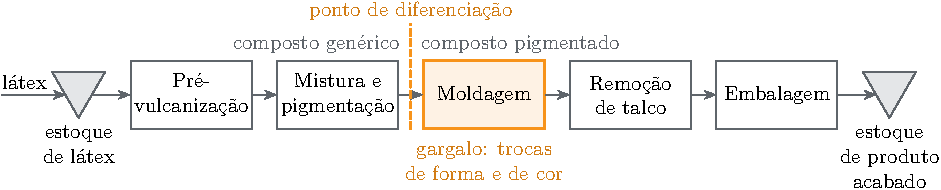
\includegraphics[page=1]{figuras/figuras.pdf}
    \fonte{Elaborado pelo autor (2026).}
\end{figure}

\section{Máquinas de moldagem e \textit{setups}}
\label{sec:maquinas}

A moldagem é feita por máquinas paralelas e independentes, com tanques, estufa e extração próprios (Figura~\ref{fig:linhas_planta}). As máquinas diferem no tamanho das formas e dos tanques, e cada uma possui taxas de produção e compatibilidades próprias para cada formato e acabamento de balão. A capacidade produtiva pode ser reduzida por ociosidades programadas, decorrentes de manutenções preventivas, reformas ou paradas não planejadas. A heterogeneidade entre equipamentos é o fator que viabiliza a operação simultânea de diferentes balões: cada máquina pode ser alocada a um formato distinto, permitindo atender o \textit{mix} sem que todas as máquinas passem por \textit{setup} ao mesmo tempo.

Cada máquina trabalha com um único formato de cada vez, mas não necessariamente com uma única cor. Nas máquinas de uma cor, a cadeia de formas gira num plano vertical, em torno de um eixo paralelo ao chão: as formas percorrem as etapas no trecho inferior e voltam vazias pelo trecho superior. Nas máquinas de duas cores, a cadeia gira num plano horizontal, em torno de um eixo perpendicular ao chão, e cada um dos dois lados passa por um tanque de composto próprio, de modo que a máquina produz duas cores ao mesmo tempo com o mesmo formato.

\begin{figure}[H]
    \centering
    \caption{Máquinas de moldagem em paralelo}
    \label{fig:linhas_planta}
    \includegraphics[page=2]{figuras/figuras.pdf}
    \fonte{Elaborado pelo autor (2026).}
\end{figure}

Nos dois tipos, a cadeia leva as formas em fila única e circula continuamente pelas etapas da máquina, mostradas para uma máquina de uma cor na Figura~\ref{fig:linha_maquina}. A cadeia mergulha as formas num banho de coagulante e, em seguida, no tanque de composto pigmentado, de onde saem recobertas por um filme de látex já na cor do composto, e as conduz por um banho de talco e pela estufa de vulcanização. Na saída da estufa, o balão passa por uma lavagem em água quente, um rolo enrola a borda do filme sobre si mesma e forma o anel da boca, e jatos de ar comprimido extraem o balão da forma e o lançam num contêiner. A forma vazia retorna ao início da cadeia e recomeça o ciclo.

\begin{figure}[H]
    \centering
    \caption{Etapas de uma máquina de moldagem de uma cor}
    \label{fig:linha_maquina}
    \includegraphics[page=3]{figuras/figuras.pdf}
    \fonte{Elaborado pelo autor (2026).}
\end{figure}

\begin{wrapfigure}[10]{r}{0.43\textwidth}
    \centering
    \caption{Disposição das formas em cadeia e em placa}
    \label{fig:cadeia_placa}
    \includegraphics[page=4]{figuras/figuras.pdf}
    \fonte{Elaborado pelo autor (2026).}
\end{wrapfigure}
A disposição em fila única distingue essa máquina das que mergulham no tanque uma placa com uma matriz de formas (Figura~\ref{fig:cadeia_placa}). Na cadeia, cada forma passa isolada por cada etapa e é vista de frente, sem outras formas atrás dela, o que dá estabilidade ao processo e permite inspecionar a linha balão a balão. A cadeia explica também a natureza dos dois \textit{setups}: trocar a cor é trocar o composto do tanque, com a limpeza do circuito, e trocar o formato é remontar o conjunto de formas da cadeia.

As trocas de formas entre balões de diferentes formatos configuram longos tempos de \textit{setup}: no limite mínimo, ocorrem entre turnos de trabalho, mas na prática se dão com intervalos de dias, dado o alto custo de tempo envolvido. A fábrica opera em três turnos diários, e a troca de forma consome parcela relevante de um turno de oito horas: na prática ela é feita na virada, quando a máquina já está parando.

A troca de cor é mais curta e ocorre dentro do turno, entre corridas do mesmo balão, mas é direcional e nem sempre possível. Passar de um tom claro para um escuro exige pouca limpeza; o caminho inverso exige muito mais, e alguns pares só se sucedem depois de uma limpeza completa do circuito, por risco de contaminação do composto. A fábrica mantém essa informação como uma matriz de tempos entre pares de cor, com células vazias marcando as transições que exigem limpeza completa.

Essa diferença de escala é o que separa as duas decisões: a forma montada numa máquina vale para o turno inteiro, e o que se sequencia dentro dele são as cores. Uma ordem de produção não atravessa a virada de turno: o que é iniciado num turno termina nele. Cada corrida respeita ainda um lote mínimo, abaixo do qual a corrida não compensa o tempo de preparação.

\section{Planejamento tático}
\label{sec:planejamento_tatico}

O planejamento tático determina o que, onde, quando e quanto produzir, balanceando estoques e garantindo o atendimento da demanda ao longo do horizonte. A demanda e o estoque são agregados por formato e acabamento dos balões; a segregação por cor, granularidade inferior, não é considerada nesta etapa.

Uma regra usual para dimensionar esse estoque é a cobertura: o planejador fixa quantos períodos de demanda futura o estoque de cada balão deve cobrir, e a diferença entre o alvo e o saldo orienta se a produção do período repõe ou consome estoque.

O plano de produção é elaborado em periodicidade semanal, com revisões eventuais conforme a necessidade operacional. É nesse nível que se decidem as trocas de forma, pela duração descrita na Seção~\ref{sec:maquinas}, e a forma montada em cada máquina fixa os balões que ela produz nas semanas seguintes.

A dificuldade desse nível é de horizonte e de volume. A produção de uma semana só se justifica pelo pico que ela antecipa, semanas adiante, e cada par de máquina e balão acrescenta uma decisão binária de preparação por semana.

[A ESCREVER: como o plano tático é elaborado hoje na fábrica e onde estão as dificuldades da prática atual.]

\section{Planejamento operacional}
\label{sec:planejamento_operacional}

O planejamento operacional desdobra o plano tático no curto prazo. Enquanto o nível tático decide quanto produzir de cada balão, o operacional decide em que turno, em que máquina e em que ordem; é nele que a cor aparece, porque é a cor que determina a limpeza entre uma corrida e a seguinte.

A unidade de decisão é o turno, a escala em que a forma montada se mantém (Seção~\ref{sec:maquinas}). O conjunto de decisões do nível operacional fica assim definido: quais operações cada máquina executa em cada turno, em que sequência, e em que quantidade.

A dificuldade desse nível é de sequência. O número de ordens possíveis cresce fatorialmente com as cores de um turno, e a direção da troca faz com que duas ordens das mesmas cores consumam capacidades diferentes.

[A ESCREVER: como a programação dos turnos é feita hoje na fábrica e onde estão as dificuldades da prática atual.]


\chapter{Demanda}
\label{sec:modelo_demanda}

\section{Natureza da demanda}
\label{sec:natureza_demanda}

O calendário de eventos que concentra o consumo (Seção~\ref{sec:mercado}) sugere uma série de demanda dominada por componente determinística, e não por um nível estacionário com ruído. Sob essa hipótese, verificada pelos testes da Seção~\ref{sec:caracterizacao_serie}, o esforço de previsão se desloca do patamar agregado para a datação e a composição de cada pico.

Esse padrão produz dois efeitos que se resolvem por decisões distintas. No agregado, a demanda alterna janelas que excedem a capacidade instalada e janelas que a subutilizam. No \textit{mix}, a composição do volume entre balões e entre cores muda de um evento para outro, de modo que um mesmo total pode corresponder a um conjunto inteiramente diferente de SKU. O primeiro efeito é de capacidade, o segundo é de alocação de máquina, e nenhum dos dois se resolve pela decisão que resolve o outro.

\section{Carteira e previsão}
\label{sec:carteira_previsao}

A demanda que alimenta essas decisões não chega por uma via única. Parte dela chega confirmada em pedidos com quantidade, cor e prazo acordados, a carteira, e o restante é previsão; as duas classes disputam a capacidade do mesmo parque de máquinas. A distinção não é nominal: a carteira não atendida no prazo é atraso, transportado adiante e ainda devido, enquanto a previsão não atendida não gera obrigação, é venda perdida do período e não se acumula. A proporção entre as duas varia ao longo do horizonte: nas semanas próximas quase toda a demanda já está vendida, e à medida que o horizonte se afasta a carteira rareia e a previsão predomina.

Essa assimetria governa também o dimensionamento do estoque. O nível adequado por balão não é uma constante, e sim a soma de uma parcela de ciclo, imposta pelo tamanho de lote, de uma parcela sazonal, que antecipa o pico, e de uma parcela de cobertura, que absorve o erro de previsão no intervalo entre duas corridas do mesmo balão. Dimensioná-las é arbitrar entre o custo de carregamento, proporcional ao capital imobilizado, e o custo da falta, medido em margem perdida e em prazo descumprido.

As duas classes não coincidem com os regimes de produção da Seção~\ref{sec:mto_mts}. O regime é atributo do SKU e decide quem carrega a parcela de cobertura: os SKU produzidos para estoque (MTS) mantêm estoque contra o erro de previsão, os demais (MTO) só têm estoque como carteira antecipada, e um SKU MTS também recebe pedidos em carteira.

\section{Dados históricos}
\label{sec:dados_historicos}

O histórico de vendas é o faturamento mensal da fábrica, em quilogramas, por balão, de janeiro de 2024 a maio de 2025: 17 meses, pouco mais de um ciclo anual. São 17 balões em 14 formatos, dos quais três têm dois acabamentos e os demais um só. O histórico admite assim três níveis de agregação, o total da fábrica, o formato e o balão.

\section{Caracterização da série}
\label{sec:caracterizacao_serie}

Três propriedades da série de vendas condicionam a forma do modelo de previsão, e cada uma é verificada por teste antes da estimação. A tendência é testada pelo teste de Mann-Kendall \cite{mann1945} e a sazonalidade pelo teste de Kruskal-Wallis entre os meses do ano \cite{kruskalwallis1952}. A estacionariedade é testada pelo par formado pelo teste de Dickey-Fuller \cite{dickeyfuller1979}, cuja hipótese nula é a raiz unitária, e pelo teste KPSS \cite{kwiatkowski1992}, cuja hipótese nula é a estacionariedade.

Os dois testes de estacionariedade são lidos em conjunto. As hipóteses nulas opostas separam a série estacionária da série com raiz unitária e identificam o caso em que os dados não permitem decidir. Os três testes são aplicados nos mesmos níveis de agregação em que os coeficientes são estimados.

[RESULTADOS DOS TESTES A ESCREVER]


\chapter{Previsão de demanda}
\label{sec:previsao}

\section{Modelo de previsão}
\label{sec:modelo_previsao}

A previsão é a entrada de que dependem a alocação das máquinas e, por consequência, as decisões de estoque. A modelagem proposta neste trabalho baseia-se em uma abordagem econométrica hierárquica \textit{top-down}, cuja origem é revisada na Seção~\ref{sec:revisao_previsao}. O objetivo é isolar os efeitos exógenos e sazonais em níveis agregados de histórico de vendas, onde o sinal estatístico é mais forte e o ruído é menor, e repassar esse aprendizado para os níveis mais granulares na forma de coeficientes \textit{a priori}.

O modelo extrai características (\textit{features}) exógenas e temporais através de múltiplos níveis de agregação e estima, em cada série, um nível que acompanha o patamar das vendas. O \textit{forecast} final é a recombinação desse nível com os efeitos sazonais projetados.

\begin{notacao}{Conjuntos}
$T$ & Períodos históricos.\\
$T^{\mathrm{v}} \subseteq T$ & Períodos de validação, retirados da estimação.\\
$I$ & Balões, combinações de formato e acabamento.\\
$F$ & Formatos.\\
$I_f \subseteq I$ & Balões do formato $f$.\\
$A$ & \textit{Features} exógenas e sazonais.\\
\end{notacao}

\begin{notacao}{Parâmetros}
$y_{it}$ & Demanda observada do balão $i$ no período $t$ (kg).\\
$Y_{ft}$ & Demanda observada do formato $f$ no período $t$ (kg).\\
$Y_{t}$ & Demanda observada total no período $t$ (kg).\\
$X_{at}$ & Valor da \textit{feature} $a$ no período $t$.\\
$\lambda$ & Penalização na transferência de coeficientes entre níveis.\\
$\sigma^{2}$ & Variância do passo do nível entre períodos consecutivos, escolhida por série.\\
$h$ & Horizonte de previsão, em períodos.\\
\end{notacao}

\begin{notacao}{Variáveis}
$\beta^{(0)}_{a}$ & Coeficiente global da \textit{feature} $a$.\\
$\beta^{(1)}_{fa}$ & Coeficiente do formato $f$ para a \textit{feature} $a$.\\
$\beta^{(2)}_{ia}$ & Coeficiente do balão $i$ para a \textit{feature} $a$.\\
$\hat{\beta}$ & Coeficiente já estimado no nível de agregação anterior.\\
$\ell^{(0)}_{t}$ & Nível global no período $t$, em escala logarítmica.\\
$\ell^{(1)}_{ft}$ & Nível do formato $f$ no período $t$, em escala logarítmica.\\
$\ell^{(2)}_{it}$ & Nível do balão $i$ no período $t$, em escala logarítmica.\\
$\hat{d}_{i,t+h}$ & Previsão do balão $i$ para o período $t+h$ (kg).\\
\end{notacao}


A extração dos efeitos sazonais e exógenos é feita em cascata. O modelo utiliza uma formulação log-linear (multiplicativa) em detrimento de uma abordagem aditiva devido à natureza da propagação da demanda, dominada pela componente sazonal verificada na Seção~\ref{sec:caracterizacao_serie}. Em eventos de forte sazonalidade (final de ano, por exemplo), a demanda agregada pode triplicar. A transformação logarítmica permite que esse comportamento atue como um fator multiplicativo percentual, sendo repassado de forma coerente e proporcional para os níveis inferiores. Caso um modelo aditivo fosse empregado, um incremento absoluto capturado no nível global (um aumento sazonal de 10.000 kg, por exemplo) perderia o sentido ao ser cascateado para uma combinação específica de formato e acabamento, cuja escala natural de vendas é substancialmente menor. Ademais, a modelagem multiplicativa previne intrinsecamente a projeção de demandas negativas.

Para a estimação destes parâmetros, utiliza-se o algoritmo RLS (Seção~\ref{sec:revisao_previsao}), que atualiza os coeficientes incrementalmente a cada nova observação minimizando o erro quadrático acumulado. Os coeficientes sazonais acumulam todo o histórico, enquanto o nível de cada série segue um passeio aleatório de variância $\sigma^{2}$, de modo que uma mudança de patamar das vendas passa ao nível sem esperar que a média de todo o histórico a absorva. O valor de $\sigma^{2}$ é o que minimiza, em cada série, o erro da previsão um período à frente dentro de $T$.

Os coeficientes sazonais só são estimados quando $T$ cobre ao menos dois ciclos anuais. Com um único ciclo, cada mês é observado uma vez, e o seu coeficiente confunde o efeito do mês com a variação de patamar daquele ano; nesse caso $A$ fica vazio e a previsão se reduz ao nível.

A estimação inicial, no nível global, ocorre sobre a demanda total consolidada, com \textit{prior} nulo para os coeficientes, o que atribui efeito zero a um mês sem evidência contrária:
\begin{ceqn}
\begin{equation}
\begin{aligned}
\left( \hat{\ell}^{(0)}, \hat{\beta}^{(0)} \right) = \arg\min_{\ell, \beta} \Bigg( & \sum_{t \in T} \left( \ln(Y_t) - \ell_{t} - \sum_{a \in A} \beta_{a} X_{at} \right)^2 \\
& + \frac{1}{\sigma^{2}} \sum_{t \in T} \left( \ell_{t} - \ell_{t-1} \right)^2 + \lambda \sum_{a \in A} \beta_{a}^{2} \Bigg)
\end{aligned}
\label{eq:demanda_nivel0}
\end{equation}
\end{ceqn}

No nível de formato, os coeficientes globais $\hat{\beta}^{(0)}_a$ atuam como \textit{priors} para a estimação, e o termo de regularização $\lambda$ penaliza desvios do comportamento global:
\begin{ceqn}
\begin{equation}
\begin{aligned}
\left( \hat{\ell}^{(1)}_{f}, \hat{\beta}^{(1)}_{f} \right) = \arg\min_{\ell, \beta} \Bigg( & \sum_{t \in T} \left( \ln(Y_{ft}) - \ell_{t} - \sum_{a \in A} \beta_{a} X_{at} \right)^2 \\
& + \frac{1}{\sigma^{2}} \sum_{t \in T} \left( \ell_{t} - \ell_{t-1} \right)^2 + \lambda \sum_{a \in A} \left( \beta_{a} - \hat{\beta}^{(0)}_a \right)^2 \Bigg) \quad \forall f \in F
\end{aligned}
\label{eq:demanda_nivel1}
\end{equation}
\end{ceqn}

No nível de formato-acabamento, por fim, os coeficientes do formato respectivo atuam como \textit{priors} para o balão específico:
\begin{ceqn}
\begin{equation}
\begin{aligned}
\left( \hat{\ell}^{(2)}_{i}, \hat{\beta}^{(2)}_{i} \right) = \arg\min_{\ell, \beta} \Bigg( & \sum_{t \in T} \left( \ln(y_{it}) - \ell_{t} - \sum_{a \in A} \beta_{a} X_{at} \right)^2 \\
& + \frac{1}{\sigma^{2}} \sum_{t \in T} \left( \ell_{t} - \ell_{t-1} \right)^2 + \lambda \sum_{a \in A} \left( \beta_{a} - \hat{\beta}^{(1)}_{f,a} \right)^2 \Bigg) \quad \forall f \in F,\; i \in I_f
\end{aligned}
\label{eq:demanda_nivel2}
\end{equation}
\end{ceqn}

O \textit{forecast} para um período futuro $t+h$, com $t$ o último período de $T$, parte do nível corrente do balão e aplica os efeitos esperados:
\begin{ceqn}
\begin{equation}
\hat{d}_{i,t+h} = \exp \left( \hat{\ell}^{(2)}_{it} + \sum_{a \in A} \hat{\beta}^{(2)}_{ia} X_{a,t+h} \right) \quad \forall i \in I
\label{eq:forecast_final}
\end{equation}
\end{ceqn}

Os dois parâmetros regulam quanto cada série confia no próprio histórico. Com $\lambda \to \infty$, o balão herda a sazonalidade do formato, e com $\lambda = 0$ estima-a sozinho sobre a série curta. Com $\sigma^{2} \to 0$, o nível é constante e igual à média de todo o histórico; com $\sigma^{2}$ grande, acompanha a última observação dessazonalizada, como na previsão ingênua.

\section{Medida do erro}
\label{sec:avaliacao_previsao}

O erro da previsão é medido fora da amostra, sobre o conjunto $T^{\mathrm{v}}$ de períodos retirados da estimação, por duas métricas complementares. O erro percentual absoluto médio (\textit{Mean Absolute Percentage Error}, MAPE) mede a magnitude do erro do balão $i$:
\begin{ceqn}
\begin{equation}
\mathrm{MAPE}_{i} = \frac{100}{|T^{\mathrm{v}}|} \sum_{t \in T^{\mathrm{v}}} \frac{\left| y_{it} - \hat{d}_{it} \right|}{y_{it}} \quad \forall i \in I
\label{eq:mape}
\end{equation}
\end{ceqn}

O viés (\textit{bias}) mede a direção do erro, como fração da demanda realizada:
\begin{ceqn}
\begin{equation}
\mathrm{Bias}_{i} = \frac{\sum_{t \in T^{\mathrm{v}}} \left( \hat{d}_{it} - y_{it} \right)}{\sum_{t \in T^{\mathrm{v}}} y_{it}} \quad \forall i \in I
\label{eq:bias}
\end{equation}
\end{ceqn}

As duas métricas respondem a perguntas distintas do planejamento. O MAPE dimensiona a parcela de cobertura do estoque (Seção~\ref{sec:carteira_previsao}), porque mede quanto a demanda se afasta da previsão em qualquer direção. O viés indica erro sistemático, que a cobertura não corrige: viés positivo imobiliza capital em estoque que não gira, e viés negativo converte previsão em demanda não atendida. O MAPE não é definido em períodos de demanda nula, que são excluídos de $T^{\mathrm{v}}$ no cálculo por balão.

A medida segue uma origem rolante \cite{tashman2000}: para cada período de $T^{\mathrm{v}}$, o modelo é estimado com os períodos anteriores a ele e prevê só esse período, com $h = 1$, e a origem avança um período. O valor de $\lambda$ é o de menor MAPE numa janela anterior a $T^{\mathrm{v}}$, avaliada pelo mesmo protocolo, de modo que nenhum período de validação participa da escolha. Os resultados reportam a média de $\mathrm{MAPE}_{i}$ e de $\mathrm{Bias}_{i}$ entre as séries.

O modelo é comparado a métodos clássicos submetidos ao mesmo protocolo \cite{hyndman2021}: as previsões ingênua e ingênua sazonal, as médias móveis simples e ponderada de três períodos, a regressão linear na tendência e a suavização exponencial simples. Também entram os métodos de \citeonline{holt2004}, com tendência, e de \citeonline{winters1960}, com tendência e sazonalidade, os modelos ARIMA e SARIMA de \citeonline{box2015}, com ordens escolhidas pelo critério de Akaike corrigido, e uma rede neural do tipo perceptron multicamadas \cite{zhang1998}, treinada em conjunto sobre todas as séries a partir das últimas observações. Os métodos sazonais exigem, como o modelo proposto, dois ciclos completos de histórico.

\section{Avaliação em base de referência}
\label{sec:previsao_referencia}

O histórico da fábrica cobre pouco mais de um ciclo anual (Seção~\ref{sec:dados_historicos}), e por isso o modelo é avaliado primeiro numa base pública, em que a cascata de efeitos sazonais pode ser observada inteira. A base é a da competição M5 \cite{makridakis2022}, vendas diárias de uma rede varejista norte-americana, agregadas aqui em 63 meses, de fevereiro de 2011 a abril de 2016, numa hierarquia com o mesmo papel da hierarquia de balões: o total, três categorias de produto no lugar dos formatos e sete departamentos no lugar dos balões. O conjunto $T^{\mathrm{v}}$ são os 12 últimos meses, e a janela de escolha de $\lambda$, os 12 anteriores.

\begin{table}[H]
\centering
\small
\caption{Erro da previsão por departamento na base M5, de maio de 2015 a abril de 2016, com o modelo proposto em negrito.}
\label{tab:previsao_referencia}
\begin{tabular}{@{}lrr@{}}
\toprule
Método & MAPE (\%) & Viés (\%) \\
\midrule
\textbf{RLS hierárquico (proposto)} & \textbf{\boldmath 4,9} & \textbf{\boldmath $-$1,4} \\
Ingênuo & 6,8 & $-$1,1 \\
Ingênuo sazonal & 13,2 & $-$12,0 \\
Média móvel simples (3) & 7,0 & $-$1,9 \\
Média móvel ponderada (3) & 6,7 & $-$1,6 \\
Suavização exponencial simples & 6,6 & $-$1,3 \\
Holt & 6,5 & $-$0,3 \\
Holt-Winters & 4,7 & $-$0,6 \\
Regressão linear & 7,9 & $-$1,8 \\
ARIMA & 6,8 & $-$1,4 \\
SARIMA & 5,2 & $-$0,5 \\
Rede neural (MLP) & 6,1 & $-$1,9 \\
\bottomrule
\end{tabular}

\fonte{Elaborado pelo autor (2026), com dados de \citeonline{makridakis2022}.}
\end{table}

O modelo erra 4,9\% por departamento, abaixo dos métodos sem sazonalidade, entre 6,1\% e 7,9\%, e do SARIMA, com 5,2\%; só o Holt-Winters fica à frente, com 4,7\% (Tabela~\ref{tab:previsao_referencia}). A previsão ingênua sazonal, que repete o mesmo mês do ano anterior, erra 13,2\% com viés de $-12{,}0$\%, porque não acompanha o nível, que cresce no período.

A Figura~\ref{fig:previsao_referencia_arvore} mostra a cascata nos três níveis. O erro cresce com a desagregação, de 3,6\% no total para 3,8\% a 4,3\% nas categorias e 4,9\% em média nos departamentos, o que sustenta estimar os efeitos sazonais no agregado e repassá-los como \textit{prior}.

\begin{figure}[p]
    \centering
    \caption{Previsão do modelo proposto em cada nível da hierarquia da base M5.}
    \label{fig:previsao_referencia_arvore}
    \includegraphics[page=6]{figuras/figuras.pdf}
    \fonte{Elaborado pelo autor (2026), com dados de \citeonline{makridakis2022}. A faixa sombreada é $T^{\mathrm{v}}$.}
\end{figure}


\chapter{Modelo de otimização}
\label{sec:modelo_otimizacao}

\section{Arquitetura em dois níveis}
\label{sec:arquitetura}

O problema é resolvido em dois níveis encadeados. O nível semanal decide, para todo o horizonte de planejamento, quanto produzir de cada balão em cada máquina e em cada semana, arbitrando entre carteira e previsão. O nível operacional recebe desse plano uma única informação, a meta de estoque ao fim de cada semana detalhada, e decide, para essas semanas congeladas, o que cada máquina produz em cada turno; a ordem das corridas dentro de cada turno é decidida em seguida, por uma heurística de sequenciamento. Os dois níveis compartilham a estrutura de objetivo e de restrições e os parâmetros de custo; diferem no \textit{bucket} de tempo e no nível de agregação do produto. Na matriz da Figura~\ref{fig:matriz_stadtler}, o nível semanal ocupa o planejamento mestre, o nível por turno o planejamento da produção, e o sequenciamento a programação.

As decisões se distribuem por três escalas de tempo encaixadas, e a escolha de cada uma responde a um fenômeno físico do processo, não a conveniência de modelagem.

A semana é a escala do plano tático. É o intervalo em que a fábrica revisa o plano (Seção~\ref{sec:planejamento_tatico}) e em que a demanda é comercialmente estável o bastante para ser tratada como dado. O horizonte cobre um número de semanas suficiente para conter a subida sazonal, porque antecipar produção contra o pico é uma decisão que só existe se o modelo enxerga o pico.

O turno é a escala do plano operacional. É a menor unidade em que a fábrica organiza mão de obra e a fronteira natural das trocas de forma (Seção~\ref{sec:maquinas}). Só as primeiras semanas do plano tático são detalhadas em turnos, tantas quantas a carteira posta justificar; as demais permanecem agregadas até a revisão seguinte, num esquema de horizonte rolante.

A posição dentro do turno é a escala da sequência. Cada turno comporta um número pequeno de corridas de cor, porque o lote mínimo e o tempo de limpeza limitam quantas cabem, e a ordem entre elas é o que determina qual \textit{setup} de cor é pago. Não há escala abaixo dessa: o sequenciamento não decide instantes, decide a ordem.

A Figura~\ref{fig:arquitetura_niveis} resume a arquitetura. O nível semanal cobre todo o horizonte, por balão, e decide o lote de cada balão em cada máquina e semana, as formas a preparar e o estoque e as faltas de carteira e de previsão. O nível operacional abre as semanas detalhadas em turnos, por SKU, e decide a forma montada em cada máquina e turno, com a troca que pode atravessar turnos, e o lote de cada SKU em cada lado, com uma reserva de troca de cor por corrida; só a carteira entra nele como demanda. O sequenciamento recebe a forma montada, os lotes e as trocas de forma pendentes, e decide em cada turno e lado a ordem das corridas, a troca de cor efetiva e a antecipação de produção já planejada.

\begin{figure}[H]
    \centering
    \caption{Arquitetura de decisão em três níveis}
    \label{fig:arquitetura_niveis}
    \includegraphics[page=5]{figuras/figuras.pdf}
    \fonte{Elaborado pelo autor (2026).}
\end{figure}

O que desce da semana para o turno é uma única grandeza: a meta de estoque de cada balão ao fim de cada semana detalhada, cobrada como restrição suave em \eqref{eq:meta_semana}. O que sobe de volta, na revisão seguinte, é o estado real: estoque, carteira consumida e a configuração em que cada máquina ficou. Nos termos da Figura~\ref{fig:coordenacao_schneeweiss}, a meta de estoque é a instrução, o estado real é a reação, e a estrutura de restrições que o nível semanal compartilha com o operacional é a sua antecipação.

A escolha é deliberada e se opõe à alternativa de fixar as janelas de produção. Passar do nível semanal a alocação máquina-balão já resolvida garantiria consistência automática entre os planos, mas ao custo de tornar o nível operacional incapaz de reagir: qualquer prazo da carteira que não coubesse na janela herdada viraria atraso, sem possibilidade de realocar. Com a meta de estoque como único vínculo, o nível operacional decide livremente máquina, turno e sequência, e a consistência com o plano semanal é cobrada pelo estado terminal em vez de pelo caminho. É o esquema de metas com folga penalizada que \citeonline{bitranhaashax1981} formalizam para a desagregação em horizonte rolante, e a violação $g_{it}$ é o que impede que uma meta inatingível propague inviabilidade para o nível de baixo, no sentido apontado por \citeonline{schneeweiss2003}.

\section{Premissas}
\label{sec:premissas}

As premissas a seguir delimitam o alcance das duas formulações.

A demanda é determinística. Carteira e previsão são dadas como conhecidas em cada execução, e a previsão vem do modelo da Seção~\ref{sec:previsao}, sem atualização dentro de uma execução.

O estoque é único por balão e por SKU. Carteira e previsão são atendidas pelo mesmo estoque, e o que as distingue é a falta, como na Seção~\ref{sec:carteira_previsao}.

O \textit{setup} de forma é independente de máquina. O tempo de troca entre dois balões é o mesmo em todas as máquinas, e a diferenciação entre equipamentos está no custo horário do \textit{setup}. A troca de forma subsume a troca de cor, porque ao remontar a forma a máquina é preparada para a primeira cor do novo balão sem \textit{setup} adicional de cor.

A perecibilidade do látex não é modelada. O recebimento diário e a capacidade dos tanques são tratados como não restritivos, e a decisão de produção é limitada pela capacidade de moldagem (Seção~\ref{sec:fluxo}), não por disponibilidade de composto.

\section{Notação comum}

Os índices são fixos nos dois modelos: $i$ para balão (formato e acabamento, sem cor), $j$ para máquina, $\ell$ para lado de cor da máquina, $t$ para semana, $s$ para turno e $k$ para SKU-cor, isto é, a combinação de balão e cor. O SKU herda os parâmetros do balão a que pertence, por meio do subconjunto $K_i$ definido adiante.

\begin{notacao}{Parâmetros}
$m_{i}$ & Margem de contribuição do balão $i$ (R\$/kg).\\
$h_{i}$ & Custo de manter o balão $i$ em estoque por uma semana, Seção~\ref{sec:custo_estoque} (R\$/kg).\\
$c_{j}$ & Custo do \textit{setup} da máquina $j$ por hora (R\$/h).\\
$n_{j}$ & Número de lados de cor da máquina $j$: 1 na máquina de uma cor e 2 na de duas cores.\\
$p_{ij}$ & Produtividade do balão $i$ em cada lado da máquina $j$ (kg/h).\\
$q_{i}$ & Lote mínimo do balão $i$ (kg).\\
\end{notacao}

Os três parâmetros de custo são distintos por construção. A venda que deixa de acontecer custa a margem $m_i$; o estoque parado custa $h_i$, que remunera o capital imobilizado; e o \textit{setup} custa as horas de máquina e equipe que consome, com a energia e o composto descartado, medidas por $c_j$. O custo de oportunidade das horas de \textit{setup} não entra na função objetivo: essas horas já reduzem a capacidade disponível na restrição correspondente, e a produção que deixa de ocorrer reaparece como falta penalizada; cobrá-la também no objetivo contaria a mesma perda duas vezes.

O custo $h_i$ segue a forma $h = r\,v$ da Seção~\ref{sec:custo_estoque}, com conversão linear para a semana, $h_i = (\theta/52)\,v_i$, em que $\theta$ é a taxa anual e $v_i$ o valor unitário do balão, e é cobrado sobre o estoque de fechamento da semana, como no CLSP. A taxa $\theta$ é parâmetro de entrada, declarado e sujeito a análise de sensibilidade, não constante embutida.

\section{Modelo semanal}
\label{sec:modelo_semanal}

O nível semanal é um problema de dimensionamento de lotes capacitado em máquinas paralelas não relacionadas. O índice de dia não existe neste nível: a ordem de produção dentro da semana é decisão do nível operacional, e o \textit{setup} é cobrado por ativação de par balão-máquina na semana, independente de sequência.

O produto deste nível é o balão, sem cor, por duas razões. A troca de forma é o \textit{setup} que consome capacidade na escala da semana, enquanto a troca de cor só existe dentro do turno; e a previsão agregada por balão tem erro relativo menor que a soma das previsões por cor, porque os desvios entre cores se compensam. A cor e o destino de cada quilograma, estoque ou carteira, ficam para o nível operacional, que conhece a carteira por SKU. As duas razões são hipóteses do desenho, testáveis sobre os dados: a primeira pela comparação entre as matrizes de troca de forma e de cor, a segunda pelo MAPE da Equação~\eqref{eq:mape} calculado nos dois níveis.

A demanda entra nas duas classes da Seção~\ref{sec:carteira_previsao}, sobre um estoque único. A carteira $d_{it}$ é a parcela confirmada; a previsão entra líquida da carteira, $f_{it} = \max(0, \hat{d}_{it} - d_{it})$, com $\hat{d}_{it}$ a previsão da Seção~\ref{sec:modelo_previsao}. Como a carteira consome a previsão em toda semana, sem fronteira, $f_{it}$ tende a zero nas semanas próximas e predomina nas distantes.

\begin{notacao}{Conjuntos}
$T$ & Semanas do horizonte de planejamento.\\
$I$ & Balões.\\
$J$ & Máquinas ativas.\\
$J_{i} \subseteq J$ & Máquinas compatíveis com o balão $i$.\\
\end{notacao}

\begin{notacao}{Parâmetros}
$d_{it}$ & Carteira do balão $i$ com vencimento na semana $t$ (kg).\\
$f_{it}$ & Previsão do balão $i$ na semana $t$, líquida da carteira (kg).\\
$\bar{d}_{i}$ & Previsão semanal média dos SKU do balão $i$ produzidos para estoque (kg).\\
$\underline{I}_{i}$ & Estoque mínimo do balão $i$ (kg).\\
$\Omega$ & Capacidade do armazém (kg).\\
$\kappa_{jt}$ & Horas produtivas de cada lado da máquina $j$ na semana $t$ (h).\\
$\tau_{i}$ & Tempo de \textit{setup} do balão $i$ por preparação semanal, $\tau_{i} = \tau^{\mathrm{F}}_{i} + \tau^{\mathrm{C}}_{i}$ (h).\\
$\tau^{\mathrm{F}}_{i}, \tau^{\mathrm{C}}_{i}$ & Parcelas de forma e de cor de $\tau_{i}$ (h).\\
$I_{i0}, b_{i0}$ & Estoque e carteira em atraso do balão $i$ no início do horizonte (kg).\\
\end{notacao}

\begin{notacao}{Variáveis}
$x_{ijt} \ge 0$ & Quantidade do balão $i$ produzida na máquina $j$ na semana $t$ (kg).\\
$y_{ijt} \in \{0,1\}$ & 1 se o balão $i$ é preparado na máquina $j$ na semana $t$.\\
$I_{it} \ge 0$ & Estoque do balão $i$ ao fim da semana $t$ (kg).\\
$b_{it} \ge 0$ & Carteira do balão $i$ em atraso ao fim da semana $t$ (kg).\\
$l_{it} \ge 0$ & Venda perdida do balão $i$ na semana $t$ (kg).\\
$g_{it} \ge 0$ & Violação do estoque mínimo do balão $i$ na semana $t$ (kg).\\
\end{notacao}

O estoque mínimo dos balões produzidos para estoque é calculado antes da otimização. Ele cobre uma semana de consumo médio do horizonte, o intervalo entre duas revisões do plano, acrescida da parcela de cobertura do erro de previsão (Seção~\ref{sec:carteira_previsao}), medida pelo MAPE da Equação~\eqref{eq:mape}, e é recalculado a cada execução do horizonte rolante:
\begin{ceqn}
\begin{equation}
\underline{I}_{i} = \bar{d}_{i} \left( 1 + \frac{\mathrm{MAPE}_{i}}{100} \right) \quad \forall i \in I
\label{eq:estoque_minimo}
\end{equation}
\end{ceqn}

\noindent\textbf{Minimizar, em ordem lexicográfica, $(Z^{S}_{1}, Z^{S}_{2}, Z^{S}_{3}, Z^{S}_{4})$}
\begin{ceqn}
\begin{equation}
\begin{aligned}
Z^{S}_{1} &= \sum_{i \in I}\sum_{t \in T} m_{i}\, b_{it} \\
Z^{S}_{2} &= \sum_{i \in I}\sum_{t \in T} m_{i}\, l_{it} \\
Z^{S}_{3} &= \sum_{i \in I}\sum_{t \in T} m_{i}\, g_{it} \\
Z^{S}_{4} &= \sum_{i \in I}\sum_{j \in J_i}\sum_{t \in T} c_{j}\, \tau_{i}\, y_{ijt}
    + \sum_{i \in I}\sum_{t \in T} h_{i}\, I_{it}
\end{aligned}
\label{eq:obj_semanal}
\end{equation}
\end{ceqn}

\noindent\textbf{Sujeito a}
\begin{align}
I_{i,t-1} + \sum_{j \in J_i} x_{ijt} + b_{it} + l_{it}
    &= I_{it} + d_{it} + f_{it} + b_{i,t-1}
    && \forall\, i \in I,\; t \in T \label{eq:balanco} \\
l_{it} &\le f_{it}
    && \forall\, i \in I,\; t \in T \label{eq:folga_limite} \\
I_{it} + g_{it} &\ge \underline{I}_{i}
    && \forall\, i \in I,\; t \in T \label{eq:piso_estoque} \\
\sum_{i \in I} I_{it} &\le \Omega
    && \forall\, t \in T \label{eq:capacidade_armazem} \\
\sum_{i \in I} \left( \frac{x_{ijt}}{p_{ij}} + \bigl( n_{j}\, \tau^{\mathrm{F}}_{i} + \tau^{\mathrm{C}}_{i} \bigr)\, y_{ijt} \right)
    &\le n_{j}\, \kappa_{jt}
    && \forall\, j \in J,\; t \in T \label{eq:capacidade_semanal} \\
q_{i}\, y_{ijt} \le x_{ijt} &\le M_{ijt}\, y_{ijt}
    && \forall\, i \in I,\; j \in J_i,\; t \in T \label{eq:lote_minimo}
\end{align}

A função objetivo \eqref{eq:obj_semanal} ordena as faltas pela consequência: o atraso da carteira, pedido firme descumprido que continua devido; a venda perdida, estimativa não atendida; a violação do estoque mínimo, risco de falta futura; e só então o custo de \textit{setup} e de carregamento, este sobre o estoque ao fim de cada semana. A ordem é imposta por estágios, e não por pesos, porque nenhuma economia de \textit{setup} justifica atrasar um pedido firme. Dentro de cada estágio as faltas são valoradas à margem $m_i$, o que decide qual balão absorve a falta quando a capacidade não cobre todos. Cada estágio $e$ é resolvido com os anteriores travados no valor alcançado $Z^{S*}_{e'}$. A solução de um estágio satisfaz essas travas, de modo que o estágio seguinte é sempre viável e não troca atendimento por custo:
\begin{ceqn}
\begin{equation}
Z^{S}_{e'} \le Z^{S*}_{e'} \quad \forall\, e' < e
\label{eq:trava}
\end{equation}
\end{ceqn}

O balanço \eqref{eq:balanco} tem entradas à esquerda e saídas à direita, sobre um estoque único: o modelo decide quanto existe de cada balão, não a que pedido ou a que cor vai cada quilograma. O atraso anterior $b_{i,t-1}$ reaparece do lado da demanda e permanece devido; a venda perdida $l_{it}$ fecha a conta da semana, limitada à previsão líquida por \eqref{eq:folga_limite}, e não é transportada. Nenhuma falta é proibida, e o modelo permanece viável sob qualquer capacidade.

O estoque mínimo \eqref{eq:piso_estoque} é meta suave: a violação $g_{it}$ é admitida e cobrada no terceiro estágio, de modo que a capacidade só é gasta em estoque de segurança depois de atendidas carteira e previsão. É o estoque de segurança como meta penalizada de \citeonline{absi2009}, restrito aos balões produzidos para estoque; nos demais, $\underline{I}_i = 0$ e a restrição é inativa. O mínimo não é a regra de cobertura da Seção~\ref{sec:planejamento_tatico}: cobre só o erro da semana de reposição, e o estoque acima dele continua decidido pelo custo, porque o modelo enxerga a demanda de todo o horizonte e antecipa produção quando a capacidade aperta.

A capacidade do armazém \eqref{eq:capacidade_armazem} limita o estoque total, e sua composição é decisão do modelo: quando falta espaço, os estágios decidem o que guardar, atendimento antes de estoque mínimo e, dentro do estágio, a maior margem $m_i$. Como as metas que descem ao nível operacional são estoques do próprio plano semanal, elas já cabem no armazém.

A capacidade \eqref{eq:capacidade_semanal} converte a produção em horas pela produtividade e soma as horas de \textit{setup} de cada par ativado, tudo contra as horas disponíveis. As horas são contadas por lado de cor: a máquina de duas cores tem $2\,\kappa_{jt}$ horas-lado e produz com $p_{ij}$ em cada lado. A troca de forma interrompe a cadeia inteira e consome os $n_j$ lados, enquanto cada corrida de cor ocupa só o lado do seu tanque; por isso a forma pesa $n_j\,\tau^{\mathrm{F}}_i$ e a cor $\tau^{\mathrm{C}}_i$. Com $n_j = 1$ a restrição é a da máquina de uma cor. O lote mínimo \eqref{eq:lote_minimo} liga produção e preparação: produzir exige preparar a máquina, e preparar exige produzir ao menos $q_i$. O limitante $M_{ijt}$ é tomado como o menor valor válido entre a capacidade da máquina na semana, $n_j\,p_{ij}\,\kappa_{jt}$, e a soma da carteira ainda devida, da previsão remanescente e do estoque mínimo do balão; um $M$ frouxo degradaria a relaxação linear e, com ela, o desempenho do \textit{branch-and-bound} \cite{jansdegraeve2008}.

\section{Modelo operacional por turno}
\label{sec:modelo_turno}

O nível operacional detalha as primeiras semanas do plano com \textit{bucket} de turno e repete a estrutura do nível semanal: os mesmos estágios no objetivo e as mesmas restrições, na mesma ordem, indexadas por SKU e turno. É a adaptação do \textit{block planning} de \citeonline{gunther2014} a este processo, com o bloco fixado no turno: a forma montada vale para o turno inteiro, a troca de forma é paga na fronteira, e dentro do bloco a cor entra como corrida de SKU, sem ordem; a ordem é decidida no sequenciamento da Seção~\ref{sec:sequenciamento}.

A notação é a do nível semanal, com o turno $s$ no lugar da semana $t$ e o SKU $k$ no lugar do balão nas grandezas de demanda, produção e estoque. O conjunto $K_i$ reúne os SKU do balão $i$ e particiona $K$. O balão continua sendo a unidade da forma, e seus parâmetros passam aos seus SKU: $p_{kj} = p_{ij}$, $q_k = q_i$, $m_k = m_i$, $h_k = h_i$ e $J_k = J_i$ para todo $k \in K_i$. Variáveis indexadas por balão ou SKU e máquina existem apenas para as máquinas compatíveis.

\begin{notacao}{Conjuntos}
$T^{\mathrm{O}} \subseteq T$ & Primeiras semanas do horizonte, detalhadas em turnos.\\
$S$ & Turnos das semanas de $T^{\mathrm{O}}$, ordenados; $\bar{s}_t$ é o último turno da semana $t$.\\
$K$ & SKU, pares de balão e cor.\\
$K_{i} \subseteq K$ & SKU do balão $i$.\\
$L_{j}$ & Lados de cor da máquina $j$, $\{1, \dots, n_j\}$.\\
\end{notacao}

\begin{notacao}{Parâmetros}
$d_{ks}$ & Carteira do SKU $k$ com vencimento no turno $s$ (kg).\\
$\hat{I}_{it}$ & Meta de estoque do balão $i$ ao fim da semana $t$ (kg).\\
$\kappa_{js}$ & Horas produtivas de cada lado da máquina $j$ no turno $s$ (h).\\
$\tau^{\mathrm{F}}_{i'i}$ & Tempo de troca da forma do balão $i'$ para a do balão $i$ (h).\\
$\bar{\tau}^{\mathrm{F}}$ & Maior tempo de troca de forma (h).\\
$\tau^{\mathrm{C}}_{kk'}$ & Tempo de troca da cor do SKU $k$ para a do SKU $k'$ (h).\\
$\bar{\tau}^{\mathrm{C}}_{k}$ & Tempo reservado por corrida do SKU $k$ (h).\\
$I_{k0}, b_{k0}$ & Estoque e carteira em atraso do SKU $k$ no início do horizonte operacional (kg).\\
$y_{ij0}$ & 1 se a forma do balão $i$ está montada na máquina $j$ no início do horizonte operacional.\\
\end{notacao}

\begin{notacao}{Variáveis}
$x_{kj\ell s} \ge 0$ & Quantidade do SKU $k$ produzida no lado $\ell$ da máquina $j$ no turno $s$ (kg).\\
$y_{ijs} \in \{0,1\}$ & 1 se a forma do balão $i$ está montada na máquina $j$ no turno $s$.\\
$y^{\mathrm{C}}_{kj\ell s} \in \{0,1\}$ & 1 se o SKU $k$ tem corrida no lado $\ell$ da máquina $j$ no turno $s$.\\
$z_{i'ijs} \in [0,1]$ & 1 se a forma passa do balão $i'$ para o balão $i$ na máquina $j$ na abertura do turno $s$.\\
$I_{ks} \ge 0$ & Estoque do SKU $k$ ao fim do turno $s$ (kg).\\
$b_{ks} \ge 0$ & Carteira do SKU $k$ em atraso ao fim do turno $s$ (kg).\\
$w_{js} \ge 0$ & Horas de troca de forma pendentes na máquina $j$ ao fim do turno $s$, com $w_{j0} = 0$ (h).\\
$g_{it} \ge 0$ & Violação da meta de estoque do balão $i$ ao fim da semana $t$ (kg).\\
\end{notacao}

\noindent\textbf{Minimizar, em ordem lexicográfica, $(Z^{O}_{1}, Z^{O}_{2}, Z^{O}_{3})$}
\begin{ceqn}
\begin{equation}
\begin{aligned}
Z^{O}_{1} &= \sum_{k \in K}\sum_{s \in S} m_{k}\, b_{ks} \\
Z^{O}_{2} &= \sum_{i \in I}\sum_{t \in T^{\mathrm{O}}} m_{i}\, g_{it} \\
Z^{O}_{3} &= \sum_{j \in J}\sum_{s \in S} c_{j} \left(
        \sum_{i' \in I}\sum_{i \in I} \tau^{\mathrm{F}}_{i'i}\, z_{i'ijs}
        + \sum_{\ell \in L_j}\sum_{k \in K} \bar{\tau}^{\mathrm{C}}_{k}\, y^{\mathrm{C}}_{kj\ell s} \right)
    + \sum_{k \in K}\sum_{s \in S} \frac{|T^{\mathrm{O}}|}{|S|}\, h_{k}\, I_{ks}
\end{aligned}
\label{eq:obj_turno}
\end{equation}
\end{ceqn}

\noindent\textbf{Sujeito a}
\begin{align}
I_{k,s-1} + \sum_{j \in J_k}\sum_{\ell \in L_j} x_{kj\ell s} + b_{ks}
    &= I_{ks} + d_{ks} + b_{k,s-1}
    && \forall\, k \in K,\; s \in S \label{eq:balanco_turno} \\
\sum_{k \in K_i} I_{k\bar{s}_t} + g_{it} &\ge \hat{I}_{it}
    && \forall\, i \in I,\; t \in T^{\mathrm{O}} \label{eq:meta_semana} \\
\sum_{k \in K} I_{ks} &\le \Omega
    && \forall\, s \in S \label{eq:capacidade_armazem_turno}
\end{align}
\begin{equation}
\begin{split}
    &\sum_{k \in K} \left( \frac{x_{kj\ell s}}{p_{kj}} + \bar{\tau}^{\mathrm{C}}_{k}\, y^{\mathrm{C}}_{kj\ell s} \right) + w_{j,s-1} - w_{js} \\
    &\quad + \sum_{i' \in I}\sum_{i \in I} \tau^{\mathrm{F}}_{i'i}\, z_{i'ijs} \le \kappa_{js}
    \qquad \forall\, j \in J,\; \ell \in L_j,\; s \in S
\end{split}
\label{eq:capacidade_turno}
\end{equation}
\begin{align}
w_{js} &\le w_{j,s-1} + \sum_{i' \in I}\sum_{i \in I} \tau^{\mathrm{F}}_{i'i}\, z_{i'ijs}
    && \forall\, j \in J,\; s \in S \label{eq:troca_pendente} \\
w_{js} &\le \bar{\tau}^{\mathrm{F}} \bigl( 1 - y^{\mathrm{C}}_{kj\ell s} \bigr)
    && \forall\, k \in K,\; j \in J_k,\; \ell \in L_j,\; s \in S \label{eq:troca_concluida} \\
q_{k}\, y^{\mathrm{C}}_{kj\ell s} \le x_{kj\ell s} &\le p_{kj}\, \kappa_{js}\, y^{\mathrm{C}}_{kj\ell s}
    && \forall\, k \in K,\; j \in J_k,\; \ell \in L_j,\; s \in S \label{eq:lote_minimo_turno} \\
\sum_{i \in I} z_{i'ijs} &= y_{i'j,s-1}
    && \forall\, i' \in I,\; j \in J_{i'},\; s \in S \label{eq:forma_saida} \\
\sum_{i' \in I} z_{i'ijs} &= y_{ijs}
    && \forall\, i \in I,\; j \in J_i,\; s \in S \label{eq:forma_entrada} \\
y^{\mathrm{C}}_{kj\ell s} &\le y_{ijs}
    && \forall\, i \in I,\; k \in K_i,\; j \in J_i,\; \ell \in L_j,\; s \in S \label{eq:cor_da_forma}
\end{align}

O objetivo perde a venda perdida. Os estágios de \eqref{eq:obj_turno} são os de \eqref{eq:obj_semanal}, com a mesma trava \eqref{eq:trava}, sem o segundo: a previsão não entra neste nível, porque chega embutida na meta $\hat{I}_{it}$, e a carteira por SKU é a única demanda. O \textit{setup} é cobrado pelos tempos de troca de forma da matriz e pela reserva de cor de cada corrida, em vez do tempo médio $\tau_i$, e o carregamento semanal $h_k$ é rateado pelos turnos de cada semana.

O balanço perde a previsão. A equação \eqref{eq:balanco_turno} é \eqref{eq:balanco} por SKU e turno, sem $f$ e $l$; o atraso da carteira é transportado de um turno ao seguinte.

O estoque mínimo vira meta de fim de semana. A restrição \eqref{eq:meta_semana} exige no último turno de cada semana detalhada o estoque que o plano semanal previu para aquela semana, incluída a antecipação sazonal que ele decidiu. O nível operacional não enxerga o horizonte que justifica esse estoque, e a meta é o que o leva a produzir para ele; com a meta já coberta, a produção das semanas seguintes cai. Para balão sem SKU produzido para estoque a meta é nula: o estoque desse balão só existe como carteira antecipada. A meta é por balão: o modelo escolhe em que cores formá-la, e é nesse ponto que o equilíbrio entre estoque e carteira de cada SKU, deixado em aberto pelo nível semanal, é decidido.

O armazém é o mesmo. A restrição \eqref{eq:capacidade_armazem_turno} é \eqref{eq:capacidade_armazem} por SKU e turno.

A capacidade separa os dois \textit{setups}. Em \eqref{eq:capacidade_turno} a troca de forma entra pelas horas executadas no turno e a troca de cor pela reserva $\bar{\tau}^{\mathrm{C}}_k$ de cada corrida ativa. A restrição vale por lado de cor: na máquina de duas cores cada lado tem o seu tanque e as suas corridas, e uma troca de cor num lado não consome horas do outro. A troca de forma interrompe a cadeia inteira e entra nos dois lados, e a forma montada $y_{ijs}$ é uma só para a máquina. Como a reserva é o pior tempo de entrada na cor a partir de qualquer cor do mesmo balão, inclusive a herdada do turno anterior, qualquer ordem das corridas do turno cabe nas horas do turno. A restrição é dura: uma ordem de produção não atravessa a fronteira do turno. A troca de forma, ao contrário, pode atravessá-la: $w_{js}$ guarda as horas que faltam, \eqref{eq:troca_pendente} impede que o turno execute horas negativas, e \eqref{eq:troca_concluida} proíbe corridas enquanto a troca não termina. É o \textit{crossover} de \textit{setup} de \citeonline{belofilho2014}, sem o qual uma troca mais longa que o turno disponível nunca seria executada.

O nível semanal desconta o \textit{setup} pela mesma regra, com a troca média de forma e uma corrida de cada cor do balão, de modo que os dois níveis enxergam a mesma capacidade:
\begin{ceqn}
\begin{equation}
\tau^{\mathrm{F}}_{i} = \frac{1}{|I|} \sum_{i' \in I} \tau^{\mathrm{F}}_{i'i}, \qquad \tau^{\mathrm{C}}_{i} = \sum_{k \in K_i} \bar{\tau}^{\mathrm{C}}_{k} \quad \forall\, i \in I
\label{eq:setup_semanal}
\end{equation}
\end{ceqn}

O lote mínimo incide na corrida. A restrição \eqref{eq:lote_minimo_turno} tem a forma de \eqref{eq:lote_minimo}, com a corrida de cor no lugar da preparação semanal e a capacidade do turno de um lado como limitante.

A forma é estado. As restrições \eqref{eq:forma_saida} e \eqref{eq:forma_entrada} não têm correspondente semanal: tratam a forma montada como um fluxo entre turnos consecutivos. A forma do turno anterior sai por exatamente um arco, que a mantém, com $z_{iijs}$ e tempo nulo, ou a troca, e a forma do turno atual chega por exatamente um. Como o estado inicial tem uma forma por máquina, cada turno também tem, inclusive o ocioso; o estado sobrevive ao turno sem produção e a troca seguinte é cobrada a partir dele, o mecanismo de estado de \citeonline{soxgao1999}. Com $y$ binária, o arco entre duas formas é determinado, e $z$ pode ser contínua; as duas equações implicam $z_{i'ijs} \ge y_{i'j,s-1} + y_{ijs} - 1$, de modo que a relaxação linear é ao menos tão forte quanto a da conjunção linearizada. A restrição \eqref{eq:cor_da_forma} limita as corridas dos dois lados aos SKU da forma montada; os dois lados podem correr a mesma cor.

\section{Sequenciamento por turno}
\label{sec:sequenciamento}

O modelo operacional fixa a forma montada em cada máquina e turno e a quantidade de cada SKU em cada lado, mas não a ordem das corridas, que é decidida para cada lado de cor. Como reserva para cada corrida o pior tempo de entrada na cor, a sequência real paga menos que a reserva e deixa horas ociosas no turno. O sequenciamento ordena as corridas de cada turno e ocupa essas horas com produção já planejada para turnos futuros, como na Figura~\ref{fig:ganho_sequenciamento}.

\begin{figure}[H]
    \centering
    \caption{Reserva de troca do modelo operacional e sequência das corridas num turno}
    \label{fig:ganho_sequenciamento}
    \includegraphics[page=16]{figuras/figuras.pdf}
    \fonte{Elaborado pelo autor (2026).}
\end{figure}

O subproblema é resolvido por heurística, turno a turno, em ordem cronológica. As equações a seguir são as condições que a solução respeita. Os valores fixados pelo modelo operacional levam acento circunflexo, como $\hat{x}_{kj\ell s}$, $\hat{y}_{ijs}$ e $\hat{w}_{js}$, com $\hat{y}_{ij0} = y_{ij0}$; o estoque $I_{ks}$ segue \eqref{eq:balanco_turno} com a produção após a antecipação; os demais símbolos são os das Seções~\ref{sec:modelo_semanal} e~\ref{sec:modelo_turno}.

\begin{notacao}{Conjuntos}
$R_{j\ell s}$ & Corridas do lado $\ell$ da máquina $j$ no turno $s$, $\{k \in K : x_{kj\ell s} > 0\}$, com $\bar{n}_{j\ell s} = |R_{j\ell s}|$.\\
\noalign{\vskip 6pt}\multicolumn{2}{@{}l}{\textbf{Parâmetros}}\\[2pt]
$k_{j\ell 01}$ & SKU da cor montada no lado $\ell$ da máquina $j$ no início do horizonte operacional, única corrida do turno 0.\\
\noalign{\vskip 6pt}\multicolumn{2}{@{}l}{\textbf{Variáveis}}\\[2pt]
$x_{kj\ell s} \ge 0$ & Quantidade do SKU $k$ produzida no lado $\ell$ da máquina $j$ no turno $s$ (kg).\\
$k_{j\ell sn}$ & SKU do lado $\ell$ da máquina $j$ no turno $s$ na posição $n = 1, \dots, \bar{n}_{j\ell s}$; $k_{j\ell s0}$ é o SKU de entrada.\\
\end{notacao}

\noindent\textbf{Minimizar, em ordem lexicográfica, $(Z^{\mathrm{Q}}_{1}, Z^{\mathrm{Q}}_{2})$}
\begin{ceqn}
\begin{equation}
\begin{aligned}
Z^{\mathrm{Q}}_{1} &= \sum_{j \in J}\sum_{\ell \in L_j}\sum_{s \in S} c_{j} \sum_{n=1}^{\bar{n}_{j\ell s}} \tau^{\mathrm{C}}_{k_{j\ell s,n-1}k_{j\ell sn}} \\
Z^{\mathrm{Q}}_{2} &= \sum_{k \in K}\sum_{j \in J_k}\sum_{\ell \in L_j}\sum_{s \in S} s\, \frac{x_{kj\ell s}}{p_{kj}}
\end{aligned}
\label{eq:obj_sequenciamento}
\end{equation}
\end{ceqn}

\noindent\textbf{Sujeito a}
\begin{align}
k_{j\ell s0} &=
\begin{cases}
k_{j\ell s'\bar{n}_{j\ell s'}} & \text{se } \hat{y}_{\cdot js''} = \hat{y}_{\cdot js},\ s'' \in [s', s] \\
\varnothing & \text{caso contrário}
\end{cases}
    && \forall\, j \in J,\; \ell \in L_j,\; s \in S \label{eq:seq_entrada}
\end{align}
\begin{equation}
\begin{split}
    &\sum_{k \in R_{j\ell s}} \frac{x_{kj\ell s}}{p_{kj}} + \sum_{n=1}^{\bar{n}_{j\ell s}} \tau^{\mathrm{C}}_{k_{j\ell s,n-1}k_{j\ell sn}} + \hat{w}_{j,s-1} - \hat{w}_{js} \\
    &\quad + \sum_{i' \in I}\sum_{i \in I} \tau^{\mathrm{F}}_{i'i}\, \hat{y}_{i'j,s-1}\, \hat{y}_{ijs} \le \kappa_{js}
    \qquad \forall\, j \in J,\; \ell \in L_j,\; s \in S
\end{split}
\label{eq:seq_capacidade}
\end{equation}
\begin{align}
x_{kj\ell s} &\le p_{kj}\, \kappa_{js}\, \hat{y}_{ijs}\, [\hat{w}_{js} = 0]
    && \forall\, i \in I,\; k \in K_i,\; j \in J_i,\; \ell \in L_j,\; s \in S \label{eq:seq_forma} \\
x_{kj\ell s} &\ge q_{k}
    && \forall\, j \in J,\; \ell \in L_j,\; s \in S,\; k \in R_{j\ell s} \label{eq:seq_lote} \\
\sum_{j \in J_k}\sum_{\ell \in L_j}\sum_{s' \le s} x_{kj\ell s'} &\ge \sum_{j \in J_k}\sum_{\ell \in L_j}\sum_{s' \le s} \hat{x}_{kj\ell s'}
    && \forall\, k \in K,\; s \in S \label{eq:seq_antecipacao} \\
\sum_{k \in K} I_{ks} &\le \Omega
    && \forall\, s \in S \label{eq:seq_armazem}
\end{align}

O objetivo \eqref{eq:obj_sequenciamento} põe o bom sequenciamento antes da ocupação. O primeiro estágio minimiza o custo das trocas de cor efetivamente pagas; o segundo minimiza as horas de produção ponderadas pela ordem do turno, que caem quando a produção vem para mais cedo. Com essa ordem, a antecipação estende uma corrida de cor que já está no turno ou move uma corrida inteira, e nunca acrescenta troca de cor. O carregamento de poucos turnos não entra no objetivo.

A entrada \eqref{eq:seq_entrada} herda a cor da última corrida do turno $s'$, o último anterior a $s$ com produção no mesmo lado da máquina, ou do turno 0, inclusive através de turnos ociosos, e fica vazia depois de uma troca de forma, que já prepara a máquina para a primeira cor do novo balão: $\tau^{\mathrm{C}}_{\varnothing k} = 0$. A capacidade \eqref{eq:seq_capacidade} usa os tempos de troca efetivos da sequência. A folga entre essa capacidade e a reserva \eqref{eq:capacidade_turno} do modelo operacional é a ociosidade que a antecipação ocupa. Como cada SKU tem uma única corrida por turno, as corridas de um mesmo SKU são contíguas por construção.

A antecipação move apenas quantidade planejada e apenas para mais cedo. A forma \eqref{eq:seq_forma}, em que $[\hat{w}_{js} = 0]$ vale 1 quando a troca está concluída e 0 caso contrário, restringe a produção aos turnos em que a forma do balão está montada e pronta, em qualquer máquina compatível, e o lote mínimo \eqref{eq:seq_lote} vale para cada corrida resultante. A restrição \eqref{eq:seq_antecipacao} impede que a produção acumulada fique abaixo do plano em qualquer turno e vale com igualdade no último turno de $S$, o que preserva o total planejado; assim o estoque de cada turno nunca fica abaixo do plano operacional, o atraso não cresce e as metas de fim de semana não caem. O armazém \eqref{eq:seq_armazem} é a única restrição de estoque que a antecipação pode violar.

A heurística percorre os turnos em ordem cronológica. Em cada turno, os candidatos à antecipação são as corridas futuras dos SKU da forma montada, da mais próxima para a mais distante; a sequência é obtida por enumeração exaustiva quando o turno tem poucas corridas, e por construção gulosa seguida de busca local por troca e realocação quando tem muitas. Uma única avaliação calcula tempos, trocas e a violação de cada restrição nomeada; os movimentos não carregam regra de viabilidade, e duas soluções são comparadas pela violação total, depois por $Z^{\mathrm{Q}}_{1}$ e por $Z^{\mathrm{Q}}_{2}$.


\chapter{Resultados}
\label{sec:resultados}

\section{Previsão da demanda da fábrica}
\label{sec:resultado_previsao}

O histórico da fábrica (Seção~\ref{sec:dados_historicos}) não chega a dois ciclos anuais. Por isso o modelo de previsão opera só com o nível (Seção~\ref{sec:modelo_previsao}), e o Holt-Winters e o SARIMA ficam fora da comparação. O conjunto $T^{\mathrm{v}}$ são os meses de janeiro a abril de 2025, os mesmos cobertos pela previsão que a empresa pratica hoje, que entra na comparação como referência do planejamento atual; o restante do protocolo é o da Seção~\ref{sec:avaliacao_previsao}.

\begin{table}[htbp]
\centering
\small
\caption{Erro da previsão por balão na fábrica, de janeiro a abril de 2025, com o modelo proposto em negrito.}
\label{tab:previsao_fabrica}
\begin{tabular}{@{}lrr@{}}
\toprule
Método & MAPE (\%) & Viés (\%) \\
\midrule
\textbf{RLS hierárquico (proposto)} & \textbf{\boldmath 15,1} & \textbf{\boldmath $-$4,0} \\
Previsão da empresa & 21,0 & $-$12,9 \\
Ingênuo & 17,9 & $-$6,7 \\
Ingênuo sazonal & 25,7 & $-$13,5 \\
Média móvel simples (3) & 17,6 & 0,0 \\
Média móvel ponderada (3) & 16,5 & $-$2,3 \\
Suavização exponencial simples & 15,2 & $-$2,7 \\
Holt & 19,8 & 1,2 \\
Regressão linear & 25,9 & 13,6 \\
ARIMA & 16,2 & $-$2,0 \\
Rede neural (MLP) & 16,7 & $-$0,8 \\
\bottomrule
\end{tabular}

\fonte{Elaborado pelo autor (2026).}
\end{table}

O modelo erra 15,1\% por balão, com viés de $-4{,}0$\%, contra 21,0\% e $-12{,}9$\% da previsão praticada (Tabela~\ref{tab:previsao_fabrica}). A suavização exponencial simples tem erro equivalente, 15,2\%, o que é esperado: sem sazonalidade estimável, o modelo se reduz a um nível que se atualiza a cada mês, o mesmo princípio. O ganho sobre a prática atual está sobretudo no viés, o erro que a cobertura de estoque não corrige, reduzido a menos de um terço. Esse MAPE por balão é o parâmetro do estoque mínimo da Equação~\eqref{eq:estoque_minimo}, de modo que a redução do erro se converte diretamente em menos estoque de cobertura.


\postextual

\bibliography{referencias}

\begin{apendicesenv}
\end{apendicesenv}

\end{document}
